\RequirePackage[switch, columnwise, running, mathlines, displaymath,
mathlines]{lineno}
\RequirePackage{docswitch}
% \flag is set by the user, through the makefile:
%    make note
%    make apj
% etc.
\setjournal{\flag}

\documentclass[\docopts]{\docclass}

% You could also define the document class directly
%\documentclass[]{emulateapj}

% Custom commands from LSST DESC, see texmf/styles/lsstdesc_macros.sty
\usepackage{lsstdesc_macros}

\usepackage{graphicx}
\graphicspath{{./}{./figures/}}
\bibliographystyle{apj}

% Add your own macros here:
\newcommand{\textul}[1]{\underline{#1}}

\newcommand{\aim}[1]{\textcolor{red}{#1}}
\newcommand{\changes}[1]{\textcolor{blue}{#1}}

% in case I can think of some fancy formatting later\dots
\newcommand{\lsst}{\textsc{LSST}}
\newcommand{\plasticc}{\textsc{PLAsTiCC}}
\newcommand{\proclam}{\texttt{proclam}}
\newcommand{\snmachine}{\texttt{snmachine}}
\newcommand{\snphotcc}{\textsc{SNPhotCC}}

% ======================================================================

\begin{document}
\linenumbers

\title{The Photometric \textsc{LSST} Astronomical Time-series Classification Challenge (\textsc{PLAsTiCC}): Selection of a performance metric for classification probabilities balancing diverse science goals}

\maketitlepre

\begin{abstract}

  Light curve classification is a high priority for the of transient and variable objects, a key step in any time-domain astronomy analysis.
  However, upcoming deep photometric surveys, including the Large Synoptic Survey Telescope (\textsc{LSST}), will produce a deluge of lower signal-to-noise data for which traditional labelings are inappropriate.
  Probabilistic classifications are more appropriate for the data but are incompatible with the traditional metrics used on deterministic classifications.
  Furthermore, large survey collaborations intend to use these classification probabilities for diverse science objectives, indicating a need for a metric that balances a variety of goals.
  We describe the process used to develop an optimal performance metric for an open classification challenge that seeks probabilistic classifications and must serve many scientific interests.
  The Photometric \textsc{LSST} Astronomical Time-series Classification Challenge (\textsc{PLAsTiCC}) is an open competition aiming to identify promising methods for obtaining classification probabilities of transient and variable objects by engaging a broader community both within and outside astronomy.
  Using mock classification probability submissions mimicing archetypes of those anticipated of \textsc{PLAsTiCC}, we compare the sensitivity of two metrics of classification probabilities under various weighting schemes, finding that they yield qualitatively consistent results.
  We choose as a metric for \textsc{PLAsTiCC} a weighted modification of the log-loss because it can be more meaningfully interpreted.
  Finally, we propose extensions of our procedure to ever more complex challenge goals and suggest some guiding principles for approaching the choice of a metric of probabilistic classifications.

% Keywords are ignored in the LSST DESC Note style:
\dockeys{}

\maketitlepost

% ----------------------------------------------------------------------
% 

\section{Introduction}
\label{sec:intro}

The Large Synoptic Survey Telescope (\lsst) has the potential to advance time-domain astronomy, with anticipated impacts on the study of transient and variable objects within and beyond the Milky Way.
% Bright cosmological objects like Type Ia supernova are probes of cosmological distance (and thus the expansion of the universe).
% Core-collapse supernovae encode within their stunning demise the evolution properties of massive stars.
% Bright astrophysical transients like RR Lyrae give insight into the structure and evolution of stars.
% Active galactic nuclei probe the evolution of large massive galaxies.
% These are but some of the physical principles that are testable with the many different kinds of transients that will be delivered with the Large Synoptic Survey Telescope (LSST).
With its rapid scan strategy, exquisite depth, and many photometric filters, \lsst\ will deliver millions of time-series observations in multiple electromagnetic wavelength ranges (bands, or filters), centered on specific wavelengths of light. These are called `lightcurves' in astronomy, enabling unprecedented population-level studies of time-varying astrophysical sources.
% , in some cases across cosmic time.

Science output from the \lsst\ dataset is contingent on distinguishing classes of astrophysical sources from one another.
From obtaining population statistics of variable stars in the Milky Way to constraining the cosmological parameters with supernovae to discovering optical counterparts to multi-messenger events, accurate classifications are necessary to take advantage of the \lsst\ data volume.
The gold standard for such identification in astronomy has traditionally been based on the spectrum of the source.
However, the volume of objects anticipated of LSST, as well as potentially low signal-to-noise ratios for most sources, likely exceeds the availability of spectroscopic follow-up resources; the great majority of \lsst's time-varying discoveries will never be spectroscopically confirmed.
% Thus several science cases (such as SN cosmology) will actively depend om classification of astrophysical sources based on the photometric light curve, and possibly a much smaller training sample/model based on a spectroscopic sub-sample.
As such, there is an acute need for classifiers of photometric lightcurves that can perform well on datasets that include a wide variety of sources, and where classification over the range of objects is desired, rather than challenges that focus on only one class.

The Photometric \lsst\ Astronomical Time-series Classification Challenge (\plasticc) aims to identify and motivate the development of classification techniques that serve the astronomical community by engaging the broader community outside astronomy.
\plasticc's dataset is comprehensive and intended to encompass all the observations \lsst\ will provide in the coming years.
The simulation includes models for well-understood classes, newly observed classes, and classes that have only been proposed to exist, to simulate serendipitous discoveries anticipated of \lsst.
Additionally, \plasticc\ will join the ranks of a handful\footnote{https://www.kaggle.com/c/DarkWorlds, https://www.kaggle.com/c/galaxy-zoo-the-galaxy-challenge} of past astronomy classification challenges hosted on Kaggle\footnote{https://www.kaggle.com/competitions}, a platform for predictive modeling, that hosts data analytics competitions where seasoned professionals and amateurs alike can compete to classify, model, and predict large data sets uploaded by companies or scientific collaborations.
The Kaggle platform attracts a broad user base, and those without domain knowledge may provide novel approaches to the problem at hand.

Classification in astronomy is increasingly done based on images e.g. galaxy classification \citep{2016A&C....16...34H}, supernova classification \citep{2017ApJ...836...97C}, identifying bars in galaxies \citep{2018MNRAS.477..894A}, separating Near Earth Asteroids from artifacts in images \citep{2016PASJ...68..104M}, as well as lightcurves e.g. \citet{2016PASJ...68..104M, 2017arXiv170906257M, 2017CQGra..34f4003Z}, and even noise classification \citet{2017CQGra..34f4003Z, 2018PhRvD..97j1501G}.
Automated classification \cite{2011arXiv1110.4655D, 2012arXiv1209.1681D, 2018ApJS..236....9N,2012PASP..124.1175B} is becoming increasingly important in astronomy as the sooner one can make follow-up observations of an interesting object, the more one can learn about its underlying physical processes and nature.

Classifaction is intrinsically \textit{probabilistic} in that the goal is to \textit{constrain} the class \textit{conditioned} on limited data, thereby defining a \textit{posterior probability density}, or \textit{classification posterior} for short, over possible classes for each classified object.
Probabilities of classification that are reduced to point estimates of class become \textit{deterministic} classifications.
As an example, an object with probability $0.9$ of being in a certain class $m$ might be assigned a deterministic classification of being of class $m$, effectively rounding up the probability to $1$, yielding a point estimate of $m$ for that object.
Such a reduction of a probability density to a point estimate discards information whose impact depends on how the classification results are subsequently used.

For example, the decision of how to allocate limited spectroscopic follow-up resources could benefit from probabilistic information if provided early enough.
To reduce wasting spectroscopic resources dedicated to common class whose science use requires spectra, one might only attempt follow-up observations of the objects with the highest classification probabilities.
Spectroscopic follow-up of a rare class, on the other hand, may merit less conservative allocation; an object with even a moderate probability of being of a very rare class could be worth the risk.
% While the knowlege that an object has been identified to be a particular type with an overwhelming probability is likely different from a situation where an object is simply slightly more likely to be a particular class than the remaining classes of objects is important but could be appropriately reflected in a deterministic classifier.
% If follow-up resources were sufficiently abundant to warrant the optimization of follow-up of less well classified objects, the information in the probabilities could be useful in resource allocation.

Classification probabilities can also be propagated through a hierarchical inference of population-level parameters, enabling scientific investigations to proceed even when spectra are unavailable.
The efficacy of this application of classification probabilities has been demonstrated in the context of supernova cosmology \citep{roberts_zbeams:_2017}.
% TODO Cite all the BEAMS papers and Malz, Peters, Hlozek in prep
% Considering the different case of supernova cosmology from a photometrically classified sample of SNe, such probabilistic classifications can be propagated to subsequent analyses of cosmological parameters allowing one to extract information from the (large) part of the sample where photometric classification failed to identify a particular type with overwhelming probability \cite{roberts_zbeams:_2017}.
Thus the impact of a photometric-only survey like \lsst\ can be greatly enhanced by probabilistic classifications.
%Because of the low-signal-to-noise expected of \lsst, probabilistic classifications are more appropriate (Roberts+17) than the point estimates of previous challenges.
%Such posteriors are more valuable than point estimates, which we call deterministic classifications in this work, because of their versatility in application and encapsulation of observational and systematic error that may propagate through inference.

% A classification posterior can be propagated through population-level inference without a separate error propagation pipeline, and a probability can always be reduced to a point estimate for the purposes of decision-making (such as for allocation of follow-up resources), but a deterministic classification cannot in general be used to reconstruct a probability density for an individual object.
In light of the aforementioned benefits of classification probabilities, \plasticc\ will thus accept classifiers producing classification posteriors.\footnote{Many classifiers, including some of the most prevalent classifiers in the time-domain astronomy field, that only provide deterministic and/or binary classifications will have to convert their results to probability vectors to compete in \plasticc.}

However, probabilistic classifications are incompatible with the metrics of deterministic class assignments used in previous classification challenges \citep{kessler_supernova_2010, kessler_results_2010} and efforts to develop supernova classifiers \citep{2018ApJS..236....9N}.
In this context, a metric is simply a quantification of the performance of a classifier.
Notions of accuracy, purity, completeness, and other metrics endemic to science are examples of deterministic metrics appropriate to classification point estimates.
Many deterministic classification metrics can be modified for evaluation on probabilistic classifications \citep{lochner_photometric_2016, moller_photometric_2016, hon_deep_2017, hon_detecting_2018, 2011arXiv1108.4696G} but only by reducing class probabilities to point estimates of class and evaluating those at discrete cutoffs, the choice of which may ultimately affect the conclusions of the study.

If the data are simulated using a forward model, a metric of the accuracy of classification probabilities relative to the true, underlying types would be straightforward. However, such a simulation procedure would require beginning with a fully populated probability space over all classes and all possible lightcurves, which is an insurmountable challenge. Designing a metric to judge the performance of a classifier (and the criterion for `winning' a challange) over a set of simulated data that takes into account classification \textit{probabilities} is therefore no longer as straightforward.

%Therefore, attention must be directed toward the no longer straightforward matter of defining the criterion for a winning classifier.

In the context of astronomy, concerns about the choice of metric for probabilistic classifications have been investigated only to a limited degree thus far \citep{2018SoPh..293...28F, 2017MNRAS.464.4463K}, with most approaches concentrating on the standard metrics of purity and completeness, however metric consistency over a range of classifiers and between different analyses is not always ensured \citep{2018A&C....23...15B}. \textbf{[RH: include concrete example e.g. from SNPhotCC]}

This work explores the problem of choosing a metric of probabilistic classifications, which will be used in many science applications and thus lack a single obvious figure of merit.
The winning classifier should be robust to significant class imbalance, both between the training set and test set and within either, and other concerning systematics.

The \plasticc\ metric must be well-defined for non-binary classes, rather than the positive/negative dichotomy that are typical of metrics that have traditionally focused on detecting one type of object and separating out all other `contaminants'. Similarly, it must contain probabilistic classification information, rather than only being one label (a point estimate) of the class.

%\aim{I actually preferred the following as a list, although I agree that it could use some pruning.}
%\begin{itemize}
%\item    The metric must return a single scalar value.
%\item    The metric must be well-defined for non-binary classes.
%\item    The metric must balance diverse science use cases in the presence of heavily nonuniform class prevalence.
%\item    The metric must respect the information content of probabilistic classifications.
%\item    The metric must be able to evaluate deterministic classifications.''
%\item    The metric must be interpretable, meaning it gives a more optimal value for "good" mock classifiers and a less optimal value for mock classifiers plagued by anticipated systematic errors; in other words, it must pass basic tests of intuition.
%\item    The metric must be reliable, giving consistent results for different instantiations of the same test case.
%\end{itemize}
In order for the metric to satisfy the challenge requirements, the metric must return a single, scalar value.
It also must be reliable, giving consistent results for different simulations of the same test case.
% In addition, the metric should balance diverse science use case needs, particularly in the presence of heavily non-uniform classes.
% Deterministic classifications must be converted to probabilistic (i.e. returning a ``1'' or a ``0''), that deterministic metric must be readily convertible into a probabilistic classification - and should preserve the relationships between classes accordingly.
% Similarly, any probabilistic metric much be easily transferred to a deterministic one ( e.g. given a threshold on the most likely classficiation choice).

We perform a systematic exploration of the sensitivity of metrics of probabilistic classification to anticipated classifier failure modes using the Probabilistic Classification Metric (\proclam) code, which is is publicly available on GitHub.\footnote{\url{https://github.com/aimalz/proclam}}.
The mock classification results that we use for this exploration are described in Section~\ref{sec:data}.
The metrics we consider are presented in Section~\ref{sec:methods}.
The behavior of the metrics as a function of mock classification results is presented in Section~\ref{sec:results}.
We discuss extensions of this exploratory framework to more complex challenge goals in Section~\ref{sec:discussion}.


\section{Data}
\label{sec:data}

We explore the behavior of metrics on mock classification probabilities with isolated strengths and weaknesses as well as realistic mock classification probabilities from a publicly available lightcurve catalog.
Throughout this paper, \textit{data} always refers to mock classification submissions to \plasticc, not the \plasticc\ lightcurves; no lightcurves were simulated, viewed, or classified in the preparation of this paper.

Our data is in the form of catalogs of $N$ posterior probability vectors $p(m \mid d_{n}, D, \mathcal{C})$ over $M$ classes with labels $m$ conditioned on each observed lightcurve $d_{n}$, the training set $D$, and some parameters $\mathcal{C}$ concerning the behavior of the classifier.
We motivate $\mathcal{C}$ here before deferring its detailed explanation to later in Section~\ref{sec:mockdata}.
If a mock classifier produced $p(m \mid d_{n})$, it would take solely the lightcurve and produce a posterior over classes.
Since such a situation involves no information besides the lightcurve $d_{n}$, every classifier would produce identical classification submissions $p(m \mid d_{n})$.
Including the training set $D$ would not remedy the problem, as every classifier has access to the same training set and so would still have no way to produce different classification submissions $p(m \mid d_{n}, D)$.
Thus there must be some other parameters $\mathcal{C}$ that are specific to each classifier and contribute to the mock classification posteriors it produces.\footnote{It should be noted that classification submissions may not be derived in this way, i.e. the parameters $\mathcal{C}$ may not be explicitly known or may indicate a procedure that does not produce posteriors but, rather, scores of some kind.  However, we assume for these purposes that classifiers produce the classification posteriors \plasticc\ seeks.}
We describe below the way in which mock data is synthesized and return to the classifier parameters $\mathcal{C}$ later.

\begin{figure}
	\begin{center}
    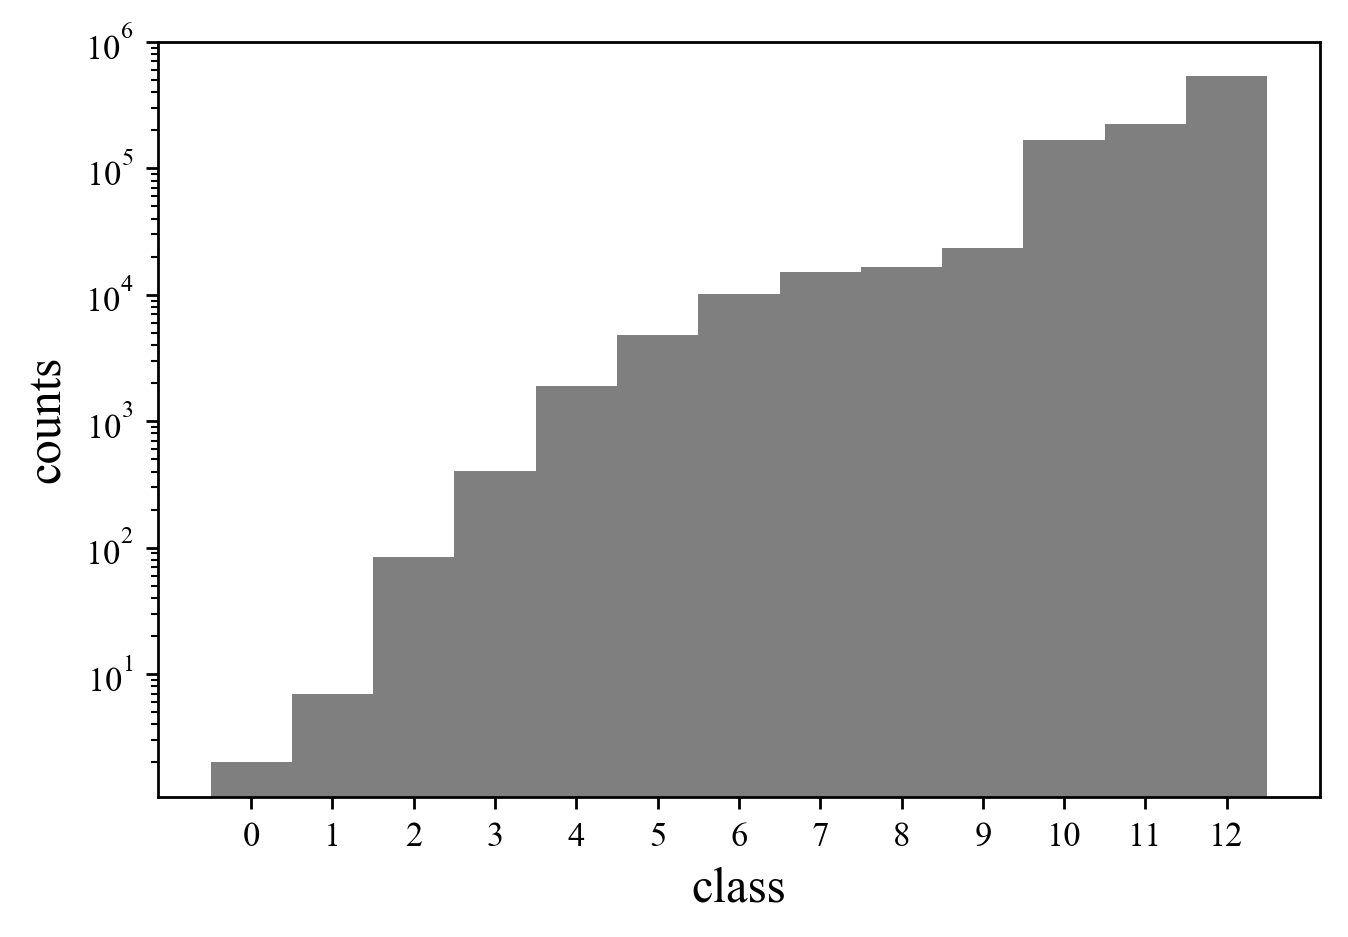
\includegraphics[width=0.49\textwidth]{./fig/complete_counts.png}
		\caption{The number of objects in a given class as shown as a function of class label, in increasing class size.
		The true classes are logarithmically distributed.}
		\label{fig:classdist}
	\end{center}
\end{figure}

As is anticipated of the real \lsst\ dataset, we use class populations that are logarithmically distributed such that they span many orders of magnitude.
%We then take $M$ draws $u_{m} \sim \mathcal{U}(0, 1)$ from the standard continuous uniform distribution and establish a discrete probability distribution $p(m) = b^{u_{m}}\ Z^{-1}$ where $Z = \sum_{m} b^{u_{m}}$, i.e. such that $\sum_{m=1}^{M} p(m) = 1$.
We take $M$ draws $u_{m'} \sim \mathcal{U}(0, 1)$ from the standard continuous uniform distribution.
These coefficients $u_{m'}$ define the discrete probability distribution $p(m') = b^{u_{m'}} / \sum_{m'} b^{u_{m'}}$ for each class $m'$ such that $\sum_{m'=1}^{M} p(m') = 1$.
% was the b in 10^b really related to the b above? This was not clear. \aim{Yes, it is the same b}
From $p(m')$ we draw $N = 10^{b}$ instances $\{m'_{n}\}$ of a true class $m'$ for each lightcurve $n$ in the catalog.
The true class membership distribution of our tests with $M = 13$ and $b = 6$ is shown in Figure~\ref{fig:classdist}.
Though the class labels for \plasticc\ are expected to be randomized, we artificially order our mock class labels by their prevalence for ease of visual interpretation.
Once the true classes have been set, mock classification probabilities for each class are derived using the procedure described in Section~\ref{sec:mockdata}.

\subsection{Mock classification schemes}
\label{sec:mockdata}

In order to observe metric performance on different classification schemes, we develop archetypical mock classifiers, devised to produce generic responses to a classification challenge without any interaction with lightcurves, images, or any other test set or training set from any challenge.
We use these mock classifiers to investigate how the performance under each metric changes in the presence of certain types of failure modes, or \textit{systematics}.
A robust metric should not reward classification schemes that display these systematic effects.
% In other words, we want a metric that deters ``gaming the system'' as much as possible.
%The cases of this section are devised to test if a metric is congruent with our intuitive understanding of what constitutes a good classifier, that it should not reward classifications suffering from the most concerning failure modes, which we will refer to as \textit{systematics} throughout the paper.
%% TODO change systematics to symptoms?
%Our impressions of systematics can be seen as reflections of the conditional probability matrix, a familiar metric of deterministic classification \citep{2012PASP..124.1175B}.

The archetypical systematics can be seen as modifications to the confusion matrix, a familiar measure of deterministic classification \citep{bloom_automating_2012}.
The confusion matrix is an $M \times M$ table of observed counts (or, if normalized, rates) of pairs of estimated class labels $\hat{m}$ (columns) and true classes $m'$ (rows) computed after a deterministic classification has been performed on some data set with $N$ objects.

Under a binary deterministic classification between positive and negative possibilities, it is natural to count the numbers of true positives $\mathrm{TP}$, false positives $\mathrm{FP}$ (Type 1 error), true negatives $\mathrm{TN}$, and false negatives $\mathrm{FN}$ (Type 2 error), which can be turned into rates relative to the true numbers of positive and negative instances; these rates may serve as building blocks for more sophisticated metrics of multi-class deterministic classifiers addressed in Section~\ref{sec:methods}.
Though probabilistic classifications are not compatible with the confusion matrix, regardless of normalization, we design tests around proposed normalized confusion matrices exhibiting various symptoms that we anticipate being problematic for \lsst.

Under a deterministic classification scheme with a normalized confusion matrix with elements $p(\hat{m}, m')$, an object with true class $m'$ would have an assigned class $\hat{m}$ drawn from $p(\hat{m} \mid m') = p(\hat{m}, m') / p(m')$, via Bayes' Rule.
We note that the elements of the confusion matrix have values of $N p(\hat{m}, m')$ and that $p(m') = N_{m'} / N$, where $N_{m'}$ is the number of true members of class $m'$, must be known in order to produce a confusion matrix.
We can thus easily obtain classification posteriors $p(\hat{m} \mid m')$ to use as the basis for classification probability submissions resulting from a confusion matrix.

Given its provenance, we refer to the matrix $\mathbb{C}$ comprised of $p(\hat{m} \mid m')$ as the \textit{conditional probability matrix} (CPM).
Without loss of generality, we can decompose $\mathbb{C}$ under some basis functions of parameters $\mathcal{C}$, the same as those introduced above in the definition of a classification posterior $p(m \mid d_{n}, D, \mathcal{C})$.
The CPM $\mathbb{C}$ thus defines the behavior of a classifier.


Since we believe the lightcurves contain information about the true class (an assumption that underlies classification as a whole), we can use the appropriate row $\mathbb{C}_{m'_{n}} = p(\hat{m} \mid m', \mathcal{C})$ of the CPM $\mathbb{C}$ as a proxy for $p(m \mid d_{n}, D, \mathcal{C})$, without directly classifying lightcurves themselves, which enabled this paper to be written without any knowledge of the \plasticc\ dataset's simulation nor validation.

To emulate the effect of natural variation of information content in different lightcurves, we generate a posterior probability vector $\vec{p}(m \mid m', \mathbb{C})$ by taking a Dirichlet-distributed draw
\begin{eqnarray}
  \label{eq:cmtoprob}
  \vec{p}(m \mid d_{n}, D, \mathcal{C}) &\sim& \mathrm{Dir}[\mathbb{C}_{m'_{n}} \delta]
	 % \frac{\mathrm{Gamma}(\mathbb{C}_{m_{n}'} \delta)}{\sum_{m'} \mathrm{Gamma}(\mathbb{C}_{m'} \delta)}
\end{eqnarray}
about $\mathbb{C}_{m'_{n}}$, with a small nonnegative perturbation factor $\delta = 0.01$.
In this way, the posterior probability vector has an expected value equal to the appropriate row in the CPM, with a variance set by $\delta$.
% \begin{eqnarray}
%  \label{eq:gamma}
%  \Gamma(\alpha) &=&
% \end{eqnarray}
We impose one restriction in addition to the normalization factor of Equation~\ref{eq:cmtoprob}, namely that all elements of $p(m \mid d_{n}, D, \mathcal{C})$ exceed $10^{-8}$, to ensure numerical stability in light of the limitations of floating point precision.

% TODO: letters for panels, refer to them in text
\begin{figure*}
	\begin{center}
    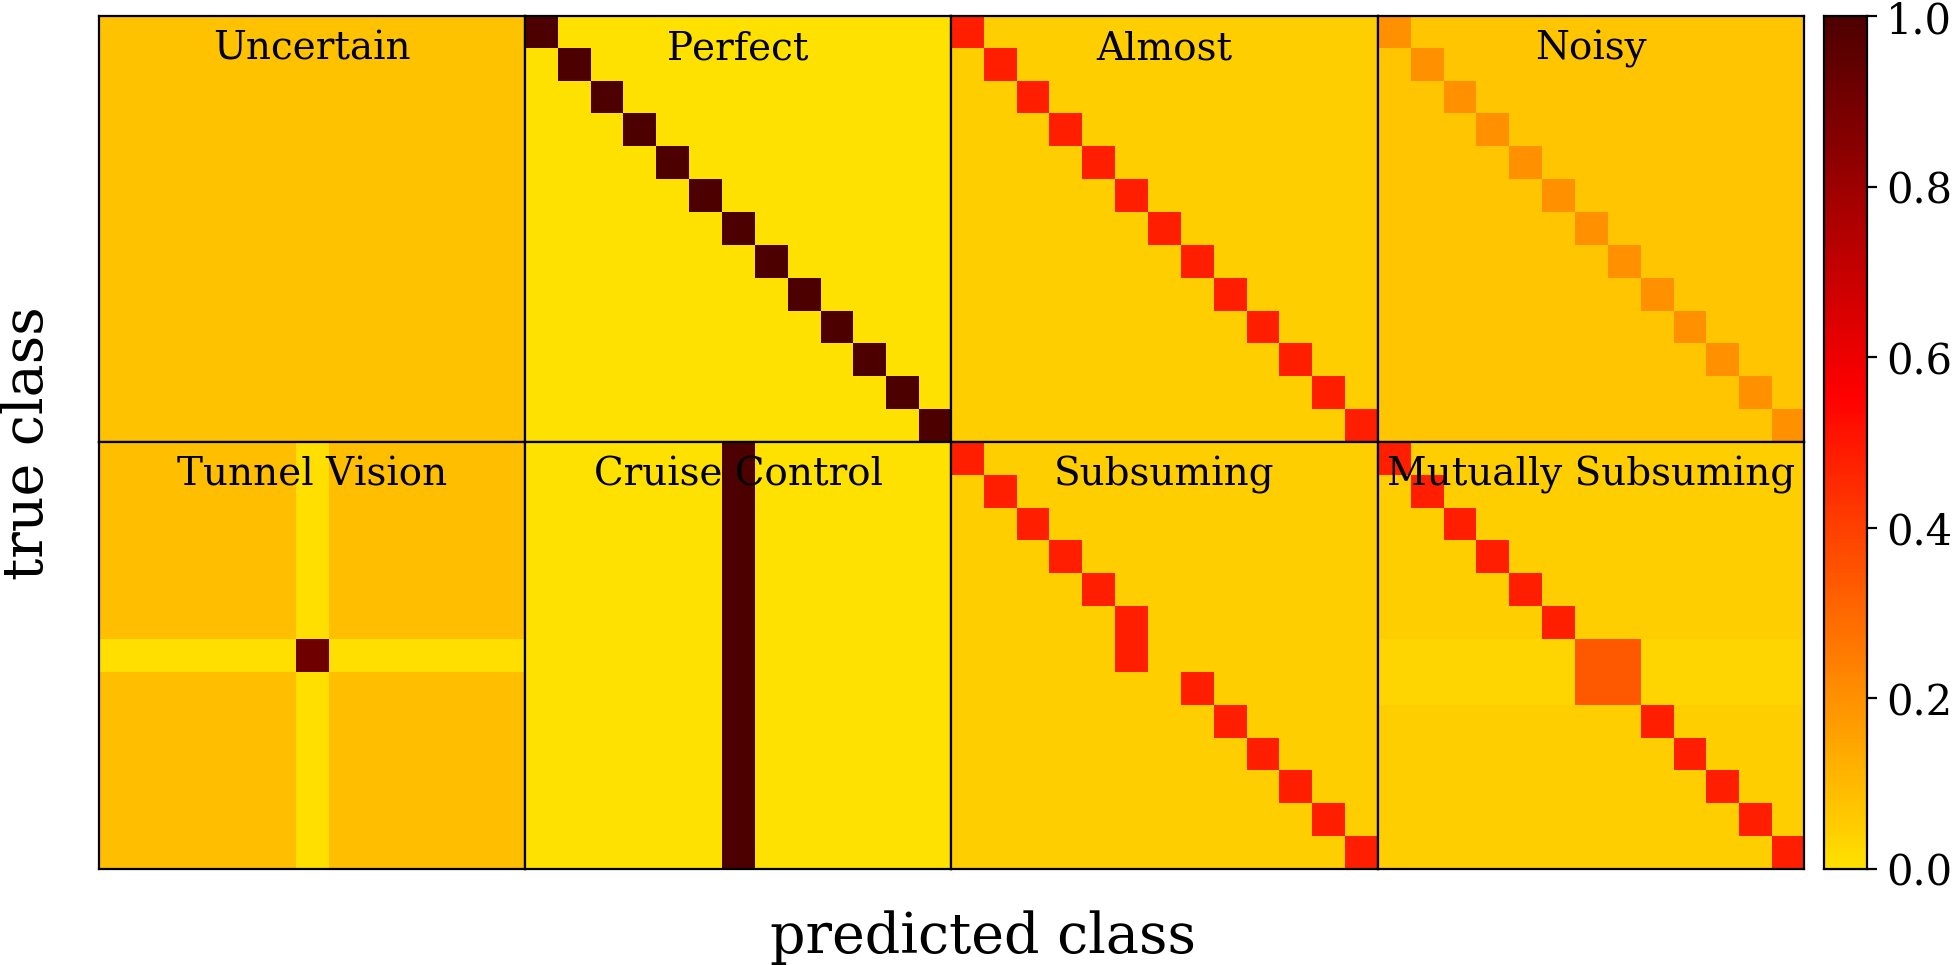
\includegraphics[width=0.8\textwidth]{./fig/all_sim_cm.png}
		\caption{Conditional probability matrices for eight mock classifiers.
		Top row:
		the uncertain classifier's uniform CPM;
		the perfect classifier's identity CPM;
		the almost perfect classifier's CPM, a linear combination of one part uniform and four parts identity;
		the noisy classifier's CPM, a linear combination of one part uniform and two parts identity.
		Bottom row:
		the tunnel vision classifier's CPM is uniform except at the row and column corresponding to one class, where it takes the values of the identity matrix;
		the cruise control classifier's CPM, which has the every row equal to a particular row of the identity;
		the subsuming classifier's CPM, which has two or more rows equal to one another;
		the mutually subsuming classifier's CPM, a symmetric case of the subsuming classifier.
		The top row shows CPMs that serve as unbiased control cases.
		The CPMs of the bottom row represent concerning systematics that we would like to ensure are not rewarded by the \plasticc\ metric.
		% The left panels show uncertain (top) and perfect (bottom) classifications, while the second panel from the left shows the almost perfect (top) and unbiased but noise (bottom) classifications. The third panel from the left illustrate the perfect classifications that generate Type 1 (False Positive) and Type 2 (False Negative) errors for one class and uniform for all others (the `tunnel classifier', top row), while the bottom row illustrates the classification where all objects are assigned to the same class (the `cruise' classifier). Finally, the panels on the far right show classifications where one class is consistently assigned to another class (subsumed to, top row), and where one consistently assigns another class to one particular class (subsumed from, bottom row). Such classifications arise when one is optimising for a particular science case (e.g., one might prioritize a tunnel classification scheme), or where one object is considered much more `valuable' to classify than others (in which case one would employ a cruise classification scheme.)
		}
		\label{fig:mock_cm}
	\end{center}
\end{figure*}

\begin{figure}
	\begin{center}
		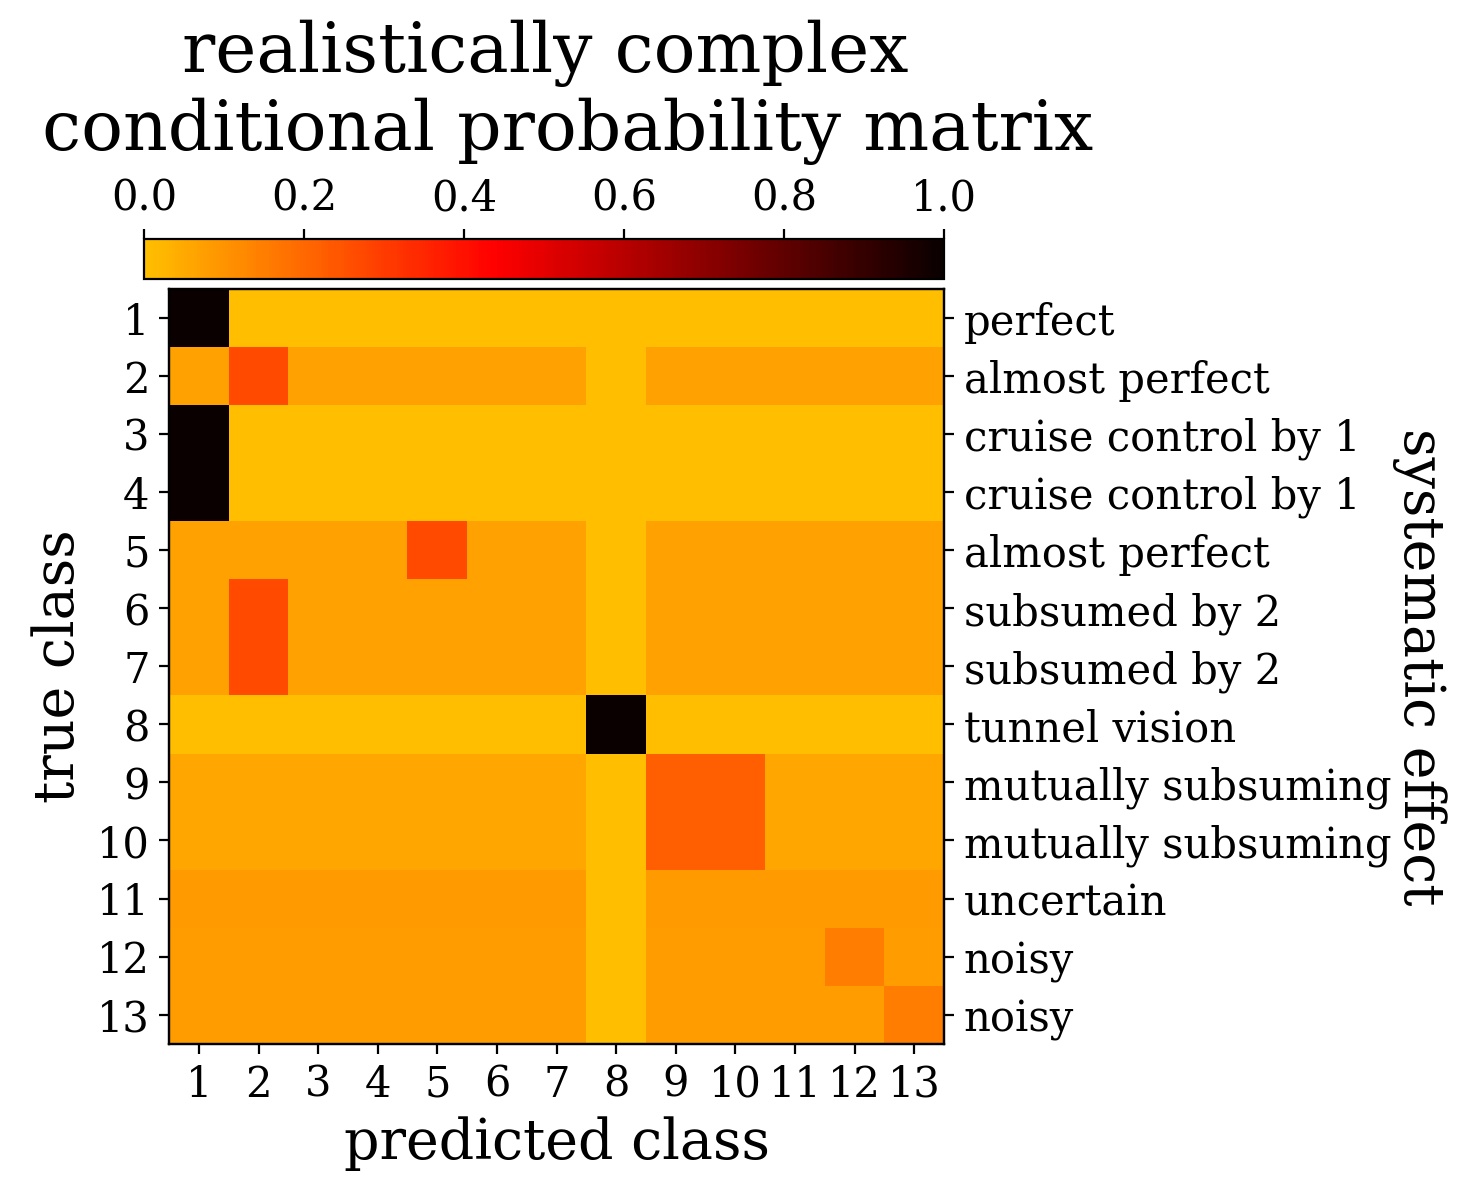
\includegraphics[width=0.49\textwidth]{./fig/combined.png}\\
    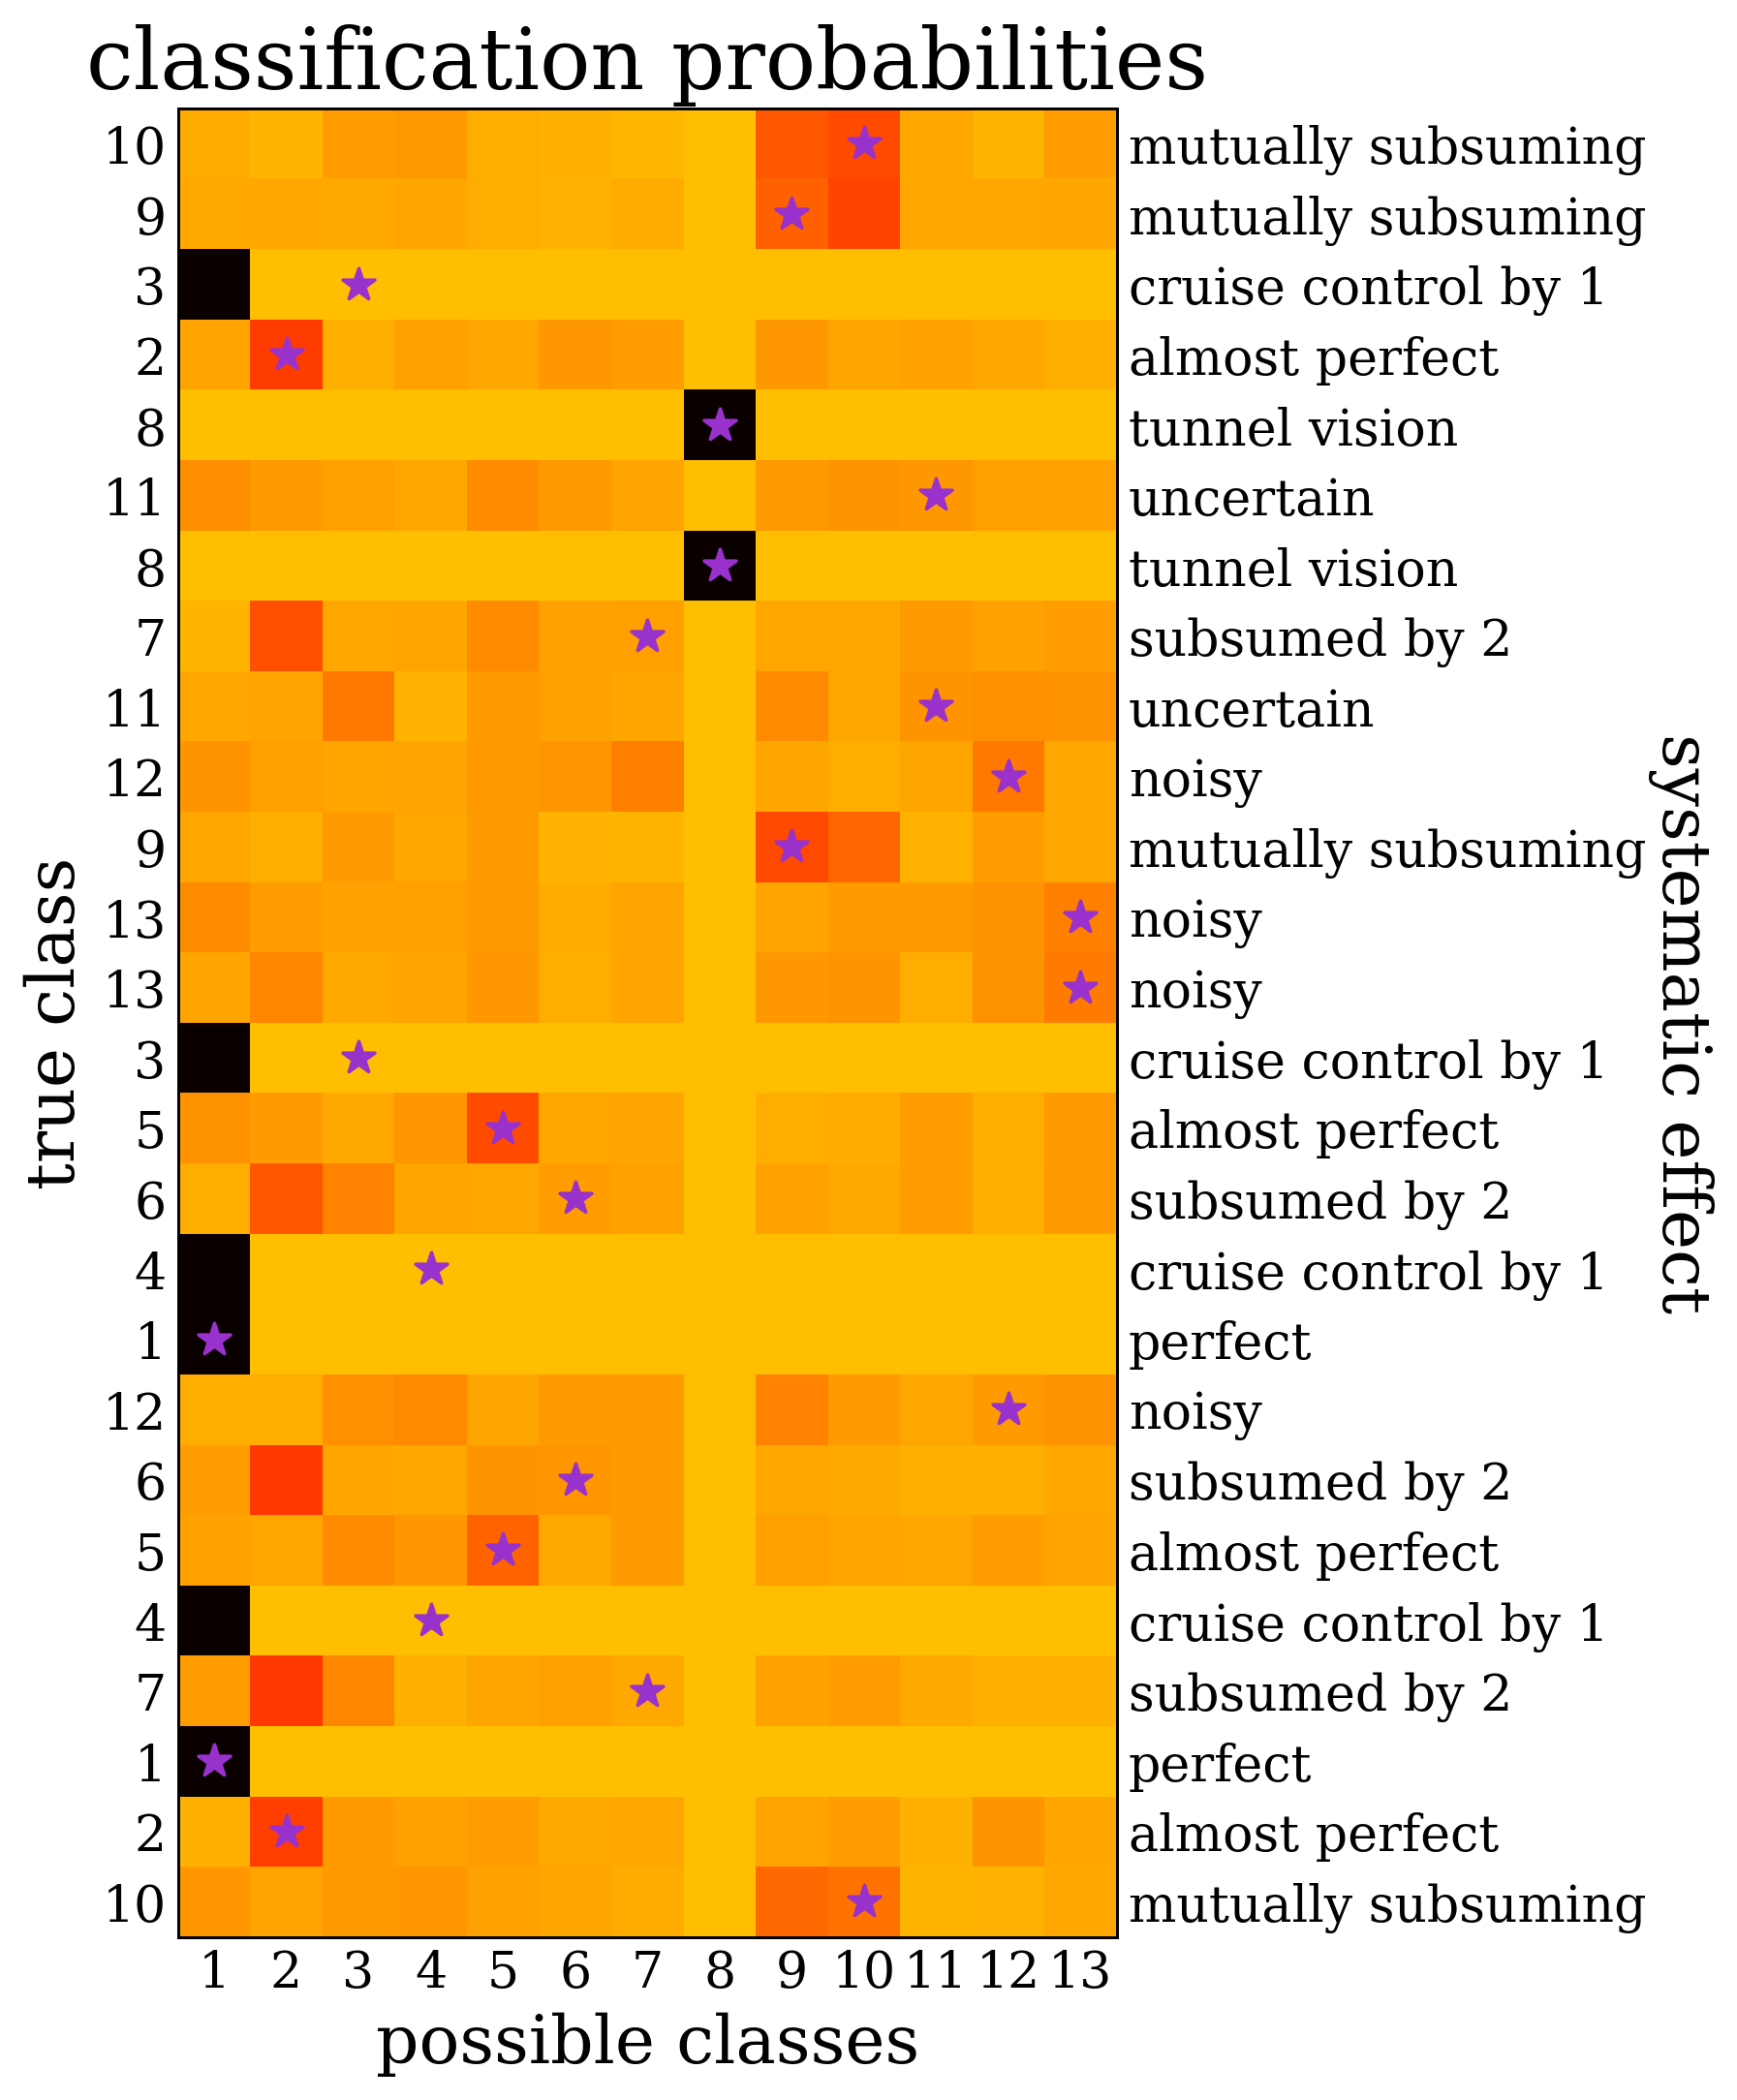
\includegraphics[width=0.49\textwidth]{./fig/examples.png}
		\caption{A realistically complex conditional probability matrix and classification posteriors drawn from it.
		Top: An example of a realistically complex conditional probability matrix, constructed by selecting a systematic for each individual class.
		This illustrates (for example), how a classifier may exhibit multiple systematics from Figure~\ref{fig:mock_cm} for each true class.
		Bottom: Example classification probabilities, drawn from the above CPM, with their true class indicated by a red star and the systematic, characterized by its row in the CPM, affecting that true class described on the right.
		The Dirichlet process emulates the variation in classification posteriors due to differences between lightcurves within a given class, leading to different classification posteriors even among rows sharing a true class.
		}
		\label{fig:mock_probs}
	\end{center}
\end{figure}

We consider eight mock classifiers, each characterized by a single systematic affecting their CPM.
Figure~\ref{fig:mock_cm} shows the CPMs corresponding to each systematic considered, discussed in detail below.
An example of a composition thereof is given in the top panel of Figure~\ref{fig:mock_probs}, as an actual classifier should be more complex than the simplified cases of Figure~\ref{fig:mock_cm}, with different behavior for each class.
To demonstrate the procedure by which mock classification posteriors are generated from rows of the CPM, we provide 22 examples of such draws in the bottom panel of Figure~\ref{fig:mock_probs}.

For each of our archetypical mock classifiers, we address:
\begin{enumerate}
  \item What characteristic behavior defines this classifier?
  \item Under what conditions does this behavior arise in real classifications?
  \item What are our expectations of and desires for response of the metric to this archetypical classifier?
\end{enumerate}

\subsubsection{Uncertain classification}
\label{sec:uncertaindata}

An entirely uniform CPM $\mathbb{U}$ (leftmost top panel of Figure~\ref{fig:mock_cm}) would correspond to uniform random guesses for deterministic classification, but, in accordance with Equation~\ref{eq:cmtoprob}, the classification posteriors are perturbations away from a uniform distribution across all classes.
The peak values of these classification posteriors will correspond to uniform random classifications, with $p(m' \mid d_{n}, D, \mathcal{C}_{\mathbb{U}}) \approx M^{-1}$.
We can consider the \textit{uncertain} classifier as an experimental control for the worst possible classification scheme, bearing in mind that if classifications were anticorrelated with true classes, the experimenter could simply reassign the classification labels to improve performance under any metric.

\subsubsection{Accurate classification}
\label{sec:accuratedata}

The \textit{perfect} classifier has a diagonal CPM $\mathbb{I}$ (left-center top panel of Figure~\ref{fig:mock_cm}), which would correspond to deterministic classifications that are always correct.
In terms of probabilistic classifications, a perfect result would be a classification posterior with 1 for the true class and 0 for all other classes.
In accordance with the classification posterior synthesis scheme of Equation~\ref{eq:cmtoprob}, the class with maximum probability is almost always still the true class, and indeed with $N \sim 10^{6}$ and $\delta = 0.01$, this is always true.
This case is also a control, in that \plasticc\ would not be necessary if we believed the perfect classifier were potentially achievable.

In addition to a perfect classifier, we test linear combinations $\mathbb{C} = (s + 1)^{-1} \left(s\mathbb{I} + \mathbb{U}\right)$ of the perfect and uncertain CPMs where the contribution of the perfect classifier is greater than that of the uncertain classifier by a factor of $s > 0$.
Deterministic classifications drawn from such a CPM would be correct $s$ times as often as they take any one wrong label, and the incorrect labels would be uncorrelated across classes.
The classification posteriors drawn from such CPMs would have some probability at classes other than the true class, but virtually all would still have their peak value at their true class.
% While $s$ would realistically be expected to vary for each class, we do not conduct a systematic investigation of this possibility at this time, and instead fix $s$ as constant for any given mock classifier.
We consider the case of the \textit{almost perfect} classifier with $s=4$ (right-center top panel of Figure~\ref{fig:mock_cm}) and the \textit{noisy} classifier with $s=2$ (rightmost top panel of Figure~\ref{fig:mock_cm}).

A classifier with different accuracy for each class may be considered a systematic in its own right.
An extreme example of such a classifier could be one with perfect classification performance on one class and uncertain classification on all others.
This classifier's CPM would be uniform except for one row, which would take a value of unity on the diagonal and zero elsewhere; if the classifier were also resilient against Type 1 errors, the CPM would also take zeros along the column in question, aside from the value of unity on the diagonal.
For many specific science applications, this type of classifier is desirable, but given the balancing of science cases within \lsst, we take a more measured approach and require that the \plasticc\ metric serve the needs of those who study a wide variety of classes for different purposes.
Hence, from the perspective of \plasticc, we seek a metric that disfavors the \textit{tunnel vision} classifier (leftmost bottom panel of Figure~\ref{fig:mock_cm}).
%However favoritism is inappropriate for the overall \plasticc\ metric, which must serve the needs of those who study all the classes and for different purposes.

\subsubsection{Inaccurate classification}
\label{sec:inaccuratedata}

Inaccurate classification in the context of a deterministic classifier is self-explanatory.
If a classifier is systematically inaccurate, its CPM has significant off-diagonal contributions.
We model inaccurate probabilistic classifications of class $m'$ by using the row of the CPM corresponding to class $\tilde{m}$ as the basis for the perturbed probability vector $p(m \mid m') = p(m \mid \tilde{m})$.
Class $m'$ is said to be subsumed by class $\tilde{m}$ for such a \textit{subsuming} classifier (right-central bottom panel of Figure~\ref{fig:mock_cm}).
The subsuming classifier may be asymmetric, or the classes may be mutually subsumed (rightmost bottom panel of Figure~\ref{fig:mock_cm}) if one already has significant off-diagonal probability, as is true for the uncertain classifier.

Subsuming is not always the mark of a poor classifier and may be insurmountable by more sophisticated classification techniques.
Real classification posteriors $p(m \mid d_{n}, D, \mathcal{C})$ are conditioned on lightcurves, training data, and assumptions necessary for the classification algorithm, and there may simply not be enough information in a lightcurve and/or training set to distinguish between classes.
% Aside from hierarchical classes, limited data can cause even wholly different physical phenomena to be indistinguishable.

For example, based on only the first few lightcurve points, it is sometimes impossible to separate cataclysmic variables, which are stars that are not destroyed and can explode many times, from supernovae, which are stars that are completely destroyed in their explosions.
Even with observations over extended periods, it can still be impossible to distinguish cataclysmic variables from active galactic nuclei that result from activity near a galaxy's central black hole.
Similarly, tidal disruption events that occur when stars are destroyed by proximity to the central black hole of a galaxy can look much like supernovae that simply happen to be near a galaxy's center.
When the prior information of the location of the source is more informative than its sparse, noisy, irregularly sampled, or short lightcurve, it may present a challenge no classifier can overcome, a fundamental limit on available information about the object.

% Subsuming is expected when distinguishing between subtypes of some class, though this failure mode is not necessarily the mark of a poor classifier.
Distinguishing between subclasses of a single phenomenon is subject to limits not only on the lightcurves of the unknown targets but also by the availability of adequate training sets.
It is nonetheless essential to identify subclasses when they have wholly different science applications.
As an example, SN Ia and SN Ibc are notorious for being difficult to distinguish.
In fact, it is more common for SN Ibc to be misclassified as SN Ia than the other way around.
This asymmetry is due to systematic underrepresentation of SN Ibc in available training sets.
However, SN Ibc contaminants in the traditional cosmology analysis done with SN Ia can bias estimates of the cosmological parameters, so the distinction is critical.

Class imbalance is a ubiquitous problem in astronomy that can severely exacerbate this form of inaccuracy, as the relative rates of various astrophysical events and objects differ by orders of magnitude from one another.
For example, RRc and RRd Lyrae stars are challenging to separate despite having different pulsation modes, and RRd stars are typically subsumed by RRc labels due to their rarity.
 % (RRc stars pulsate in the first overtone, while RRd stars pulsate simultaneously in the fundamental mode and first overtone, and are much more rare than RRc stars), and yet are challenging to separate observationally.
An extreme case of inaccurate classification is to classify all objects as the most common class (in the training or test set), a particular concern for \plasticc\ given the potential for population imbalance between classes.
Such a \textit{cruise control} classifier (left-center bottom panel of Figure~\ref{fig:mock_cm}) counters \plasticc's goal of identifying objects belonging to extremely rare classes.
We would like the \plasticc\ metric to reward a classifier that minimizes this kind of error.

\subsection{Realistic classifications}
\label{sec:realdata}

\begin{figure*}
	\begin{center}
    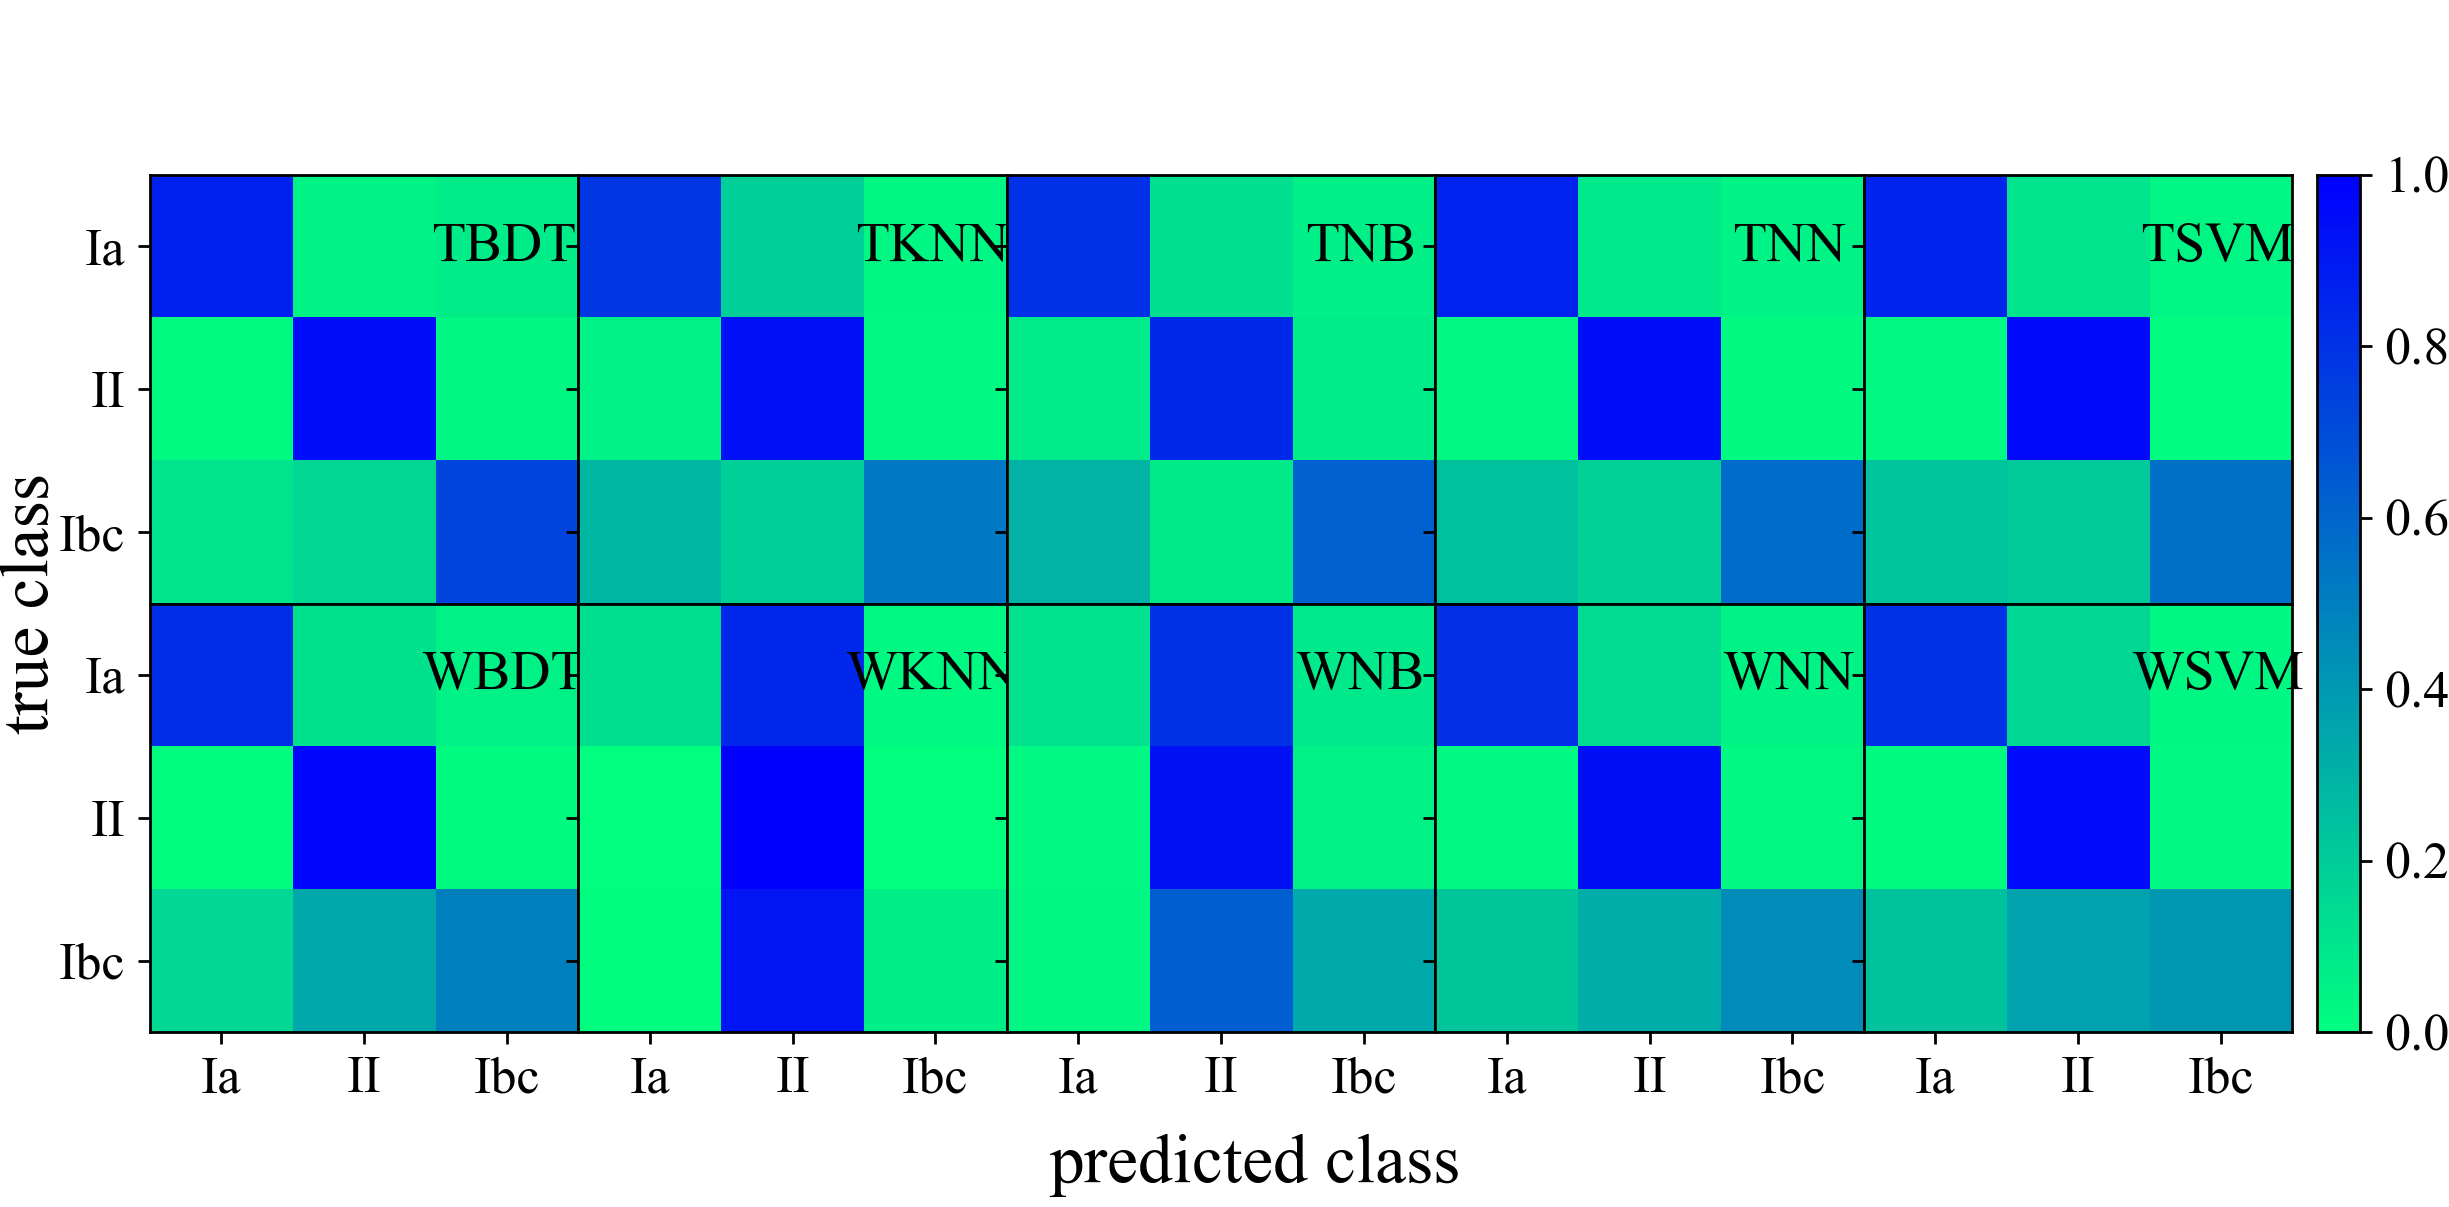
\includegraphics[width=\textwidth]{./fig/all_snphotcc_cm.png}
		\caption{Conditional probability matrices of the \citet{lochner_photometric_2016} methods applied to the \snphotcc\ dataset.
		Columns: the five machine learning methods of Boosted Decision Tree (BDT), K-Nearest Neighbors (KNN), Naive Bayes (NB), Neural Network (NN), and Support Vector Machine (SVM).
    Top row: five machine learning methods applied to template decompositions as features.
    Bottom row: the same five machine learning methods applied to wavelet decompositions as features.
		These CPMs derived from the dataset of a precursor lightcurve classification challenge by modern methods exhibit some of the systematics identified in Section~\ref{sec:mockdata} and Figure~\ref{fig:mock_cm}, particularly cruise control (WKNN, WNB), noisy (class Ibc in all but TBDT and WKNN), and perfect (class II in all).
		}
		\label{fig:snphotcc_cm}
	\end{center}
\end{figure*}

%\aim{This would be more meaningful if we were given the conditional probability matrices of actual submissions to \snphotcc\ and then checked whether the \plasticc\ metric would have designated a different winner.
%Also, it may be more interpretable if we instead use Ashish's conditional probability matrices that have more classes.}

In order to understand the performance of classifiers on simulated datasets approximating reality, we calculate the values of our metric candidates on representative classifiers of a precursor lightcurve classification challenge.
The Supernova Photometric Classification Challenge (\snphotcc) \citep{kessler_supernova_2010} focused on deterministically classifying a heterogenous population of supernovae into subclasses of SN Ia, SN II, and SN Ibc
The \snphotcc\ attracted diverse classification approaches, encompassing $\chi^{2}$ fits of the supernova lightcurves to publicly available templates \citep{nugent_kcorrections_2002}, physical models \citep{conley_sifto:_2008}, and empirical models, as well as alternatives to curve-fitting such as outlier identification on the training set Hubble diagram, dimensionality reduction, and clustering.
% TODO cite InCA?
% A general light curve shape (rather than one motivated by the physical differences between SNeIa and core collapse SNe) was assumed by some competitors and then a kernel density estimation was performed over the fit parameters, with various approaches employed including boosting over the feature space.
Machine learning was also employed, using features such as the light-curve slopes to produce a predictive model for the training data.
% TODO need citations of ML submissions to SNPhotCC
%, which are prone to bias given non-representativity of the test data and agnostic
\snphotcc\ attracted physically motivated template-based methods as well as those based on decomposition of the light curves into generic features at risk of neglecting available physical information.

Since the conclusion of the \snphotcc, the lightcurves became a testbed for a suite of machine learning classifiers.
We consider a collection of probabilistic classification methods, as presented in \citet{lochner_photometric_2016}, whose CPMs\footnote{The classifiers of \citet{lochner_photometric_2016} are indeed probabilistic but are reduced to confusion matrices via deterministic labels for this visualization and the science-motivated metric of Section~\ref{sec:science}.
In all other instances, the classification posteriors are used directly.} are shown in Figure~\ref{fig:snphotcc_cm}.
The set of classification algorithms includes template-based classification procedures, denoted as T, (\citet{sako_photometric_2011}, top row) and a wavelet decomposition, denoted as W, of the lightcurves to construct the features over which to classify (\citet{newling_statistical_2011}, bottom row), each paired with Boosted Decision Tree (BDT), K-Nearest Neighbors (KNN), Naive Bayes (NB), Neural Network (NN), and Support Vector Machine (SVM) machine learning algorithms (columns).
While the complexity of entries to the \snphotcc\ was greater than this subset, we use these examples to establish the behavior of our metrics on realistic classification submissions.

We draw attention to the marked presence of the systematics introduced in Section~\ref{sec:mockdata} in the CPMs of Figure~\ref{fig:snphotcc_cm}.
Note that the WNN and WNB methods both suffer from the cruise control systematic on SN II; it should come as no surprise that SN II are more prevalent in the \snphotcc\ dataset.
Nearly all the others exhibit classifications that are almost perfect for SN Ia, perfect for SN II, and noisy for SN Ibc.
A likely cause for this effect is that SN Ibc are poorly represented in training and template sets.
% \subsubsection{Unknown dataset}
% \label{sec:mystery}
%
% \begin{figure*}
% 	\begin{center}
% 		\includegraphics[width=0.3\textwidth]{./fig/Unknown_MLPNeuralNet_cm.png}
% 		\includegraphics[width=0.3\textwidth]{./fig/Unknown_KNeighbors_cm.png}
% 		\includegraphics[width=0.3\textwidth]{./fig/Unknown_RandomForest_cm.png}
% 		\caption{}
% 		\label{fig:unknown_cm}
% 	\end{center}
% \end{figure*}


\section{Methods}
\label{sec:methods}

%\begin{itemize}
%\item    The metric must return a single scalar value.
%\item    The metric must be well-defined for non-binary classes.
%\item    The metric must balance diverse science use cases in the presence of heavily nonuniform class prevalence.
%\item    The metric must respect the information content of probabilistic classifications.
%\item    The metric must be able to evaluate deterministic classifications.
%\item    The metric must be interpretable, meaning it gives a more optimal value for "good" mock classifiers and a less optimal value for mock classifiers plagued by anticipated systematic errors; in other words, it must pass basic tests of intuition.
%\item    The metric must be reliable, giving consistent results for different instantiations of the same test case.
%\end{itemize}

To optimally discriminate between classification techniques, there must be a performance metric, a single scalar value quantifying how appropriate a classifier is for the task at hand.
Choosing a metric for \plasticc\ therefore is logically entwined with the challenge goals.

The goal of \snphotcc\ was to identify good classifiers of SN Ia used for a photometric cosmology analysis, which lends itself to a metric that optimizes the purity of any resultant data set.
The goals of \plasticc\ are not tied to one application or even one class of transient or variable star; as such, the choice of a metric is not simple for \plasticc's diverse science goals.

%The goal of \snphotcc\ was to identify good classifiers of photometrically identified SN Ia used for cosmology analysis.
%The classifiers were ranked using a metric that optimizes the purity of any resultant data set.
%\plasticc, on the other hand, differs from \snphotcc\ in that its goals are not tied to one application or even one type of transient or variable class.
%As such, the choice of a metric is not so simple for \plasticc's diverse science goals.

%he posterior probabilities of class must be accurate for use in inference, and they must be evaluated in a way that does not excessively favor any one science application.

In Section~\ref{sec:deterministic}, we review familiar classification metrics in astronomy.
In Section~\ref{sec:probabilistic}, we introduce metrics appropriate for probabilistic classification.
We take weighted averages of the per-object metrics with per-class weights described in Section~\ref{sec:weights}.

\subsection{Deterministic metrics}
\label{sec:deterministic}

We begin with a presentation of a subset of classification metrics that have been used in the evaluation of astronomical light curve classifiers in the recent past.
The metrics we highlight make use of the notions of true positive, false positive, and false negative counts from binary deterministic classification.
We briefly define the \textit{efficiency} $\epsilon \equiv \mathrm{TP} / (\mathrm{TP} + \mathrm{FN})$ and \textit{purity} $\pi \equiv \mathrm{TP} / (\mathrm{TP} + \mathrm{FP})$.

%\subsubsection{Science-motivated metrics}
%\label{sec:science}

The goal of the \snphotcc\ was to identify one particular type of astrophysical source, SN Ia, for a single scientific application, cosmology.
% The original metric was based solely on correctly classifying SN Ia deterministically, with no penalty for confusing SN II for SN Ibc and vice versa, nor was there any notion of a confidence in a classification.
As the \snphotcc\ was only concerned with SN Ia cosmology, it was effectively binary, in that the metric did not distinguish between non-Ia classes.
The \snphotcc\ metric $\mathcal{FOM} \equiv \epsilon \cdot \tilde{\pi}$,
% \begin{eqnarray}
%   \label{eq:snphotccfom}
%   \mathcal{FOM} &\equiv& \epsilon \times \tilde{\pi}
% \end{eqnarray}
is the product of the efficiency
% \begin{eqnarray}
%   \label{eq:efficiency}
%   \epsilon_{Ia} &=& \frac{N_{Ia}^{\mathrm{true}}}{N_{Ia}^{TOT}}
% \end{eqnarray}
of SN Ia classification and a modification $\tilde{\pi} \equiv \mathrm{TP} / (\mathrm{TP} + r \mathrm{FP})$ of the purity in terms of a penalty factor $r,$
% \begin{eqnarray}
%   \label{eq:pseudopurity}
%   \tilde{P}_{Ia} &=& \frac{N_{Ia}^{\mathrm{true}}}{N_{Ia}^\mathrm{true} + W_{Ia}^\mathrm{false}N_{Ia}^\mathrm{false}}
% \end{eqnarray}
% with an additive penalty term with weight $W_{Ia}^\mathrm{false}$
motivated by the potential impact on cosmological parameter constraints due to contamination of the SN Ia sample by non-Ia classes. The pseudo-purity can be interpreted as the traditional purity when $r = 1$ as it is related to the size of the spectroscopic sample; for the \snphotcc, $r=3$ was used.

% The \snphotcc\ was related to the size of the spectroscopic subsample as roughly $w = 1 + \epsilon_{spec}^{-1} \gg 1$ but the conservative limit of $W_{Ia}^\mathrm{false} = 3$ was chosen.
%chose $r = 3$ based on a conservative limit on the acceptable amount of spectroscopic follow-up resources to waste on non-Ia targets.
% on 
% to penalize wasted spectroscopic time over rejected SNe.

% \subsection{Modified deterministic metrics}
% \label{sec:auc}

% \aim{TODO: write about AUC so it can be included in results since Michelle calculated it for us!}
% While commonly-used metrics like Receiver Operator Characteristic (ROC) curve (which maps the true positive rate against the false positive rate) and the area under the curve (AUC) can be used to infer probabilities from such classifiers, the fact that \plasticc\ is by construction simulating multiple types of objects makes the extension of ROC as a metric infeasible.

\subsection{Probabilistic metrics}
\label{sec:probabilistic}

In contrast to \snphotcc's single goal of optimal deterministic classification of a single class, \plasticc\ seeks to identify classifiers that produce classification posteriors.
We consider two metrics of classification probabilities that avoid reducing probabilities to deterministic labels.
%These metrics require additioare somewhat more involved than those of Section~\ref{sec:deterministic}, requiring additional infrastructure.

% \aim{TODO: will need to fix indexing at 0 in plots!}
Our probabilistic metrics are composed of quantities defined for each possible class $m$ available to light curve $n$, which is a true member of the set $\mathbb{S}_{m'}$ of astrophysical sources of class $m'$.
The metric value $Q_{n} = \sum_{m=1}^{M} Q_{n, m}$ for a single light curve $n$ is a sum of the per-class per-light curve metric values $Q_{n, m}$.
The metric value $Q_{m'} = \sum_{n \in \mathbb{S}_{m'}} Q_{n}$ for an entire class $m'$ is the sum of the per-light curve metrics.
Section~\ref{sec:weights} discusses how the global metrics are derived from the per-class metrics $Q_{m'}$.

As part of the derivation of the per-class per-light curve metrics, we also define the indicator (dummy) variable
\begin{eqnarray}
  \label{eq:indicator}
  \tau_{n, m} &\equiv& \begin{cases}
  0 & m' \neq m\\
  1 & m' = m
  \end{cases}
\end{eqnarray}
that indicates if an object has been correctly classified as its true type.
\subsubsection{Log-loss}
\label{sec:logloss}

The log-loss is a quantity borrowed from information theory and is related to a notion of \textit{entropy} $H_{n} = - \sum_{m=1}^{M} p(m \mid d_{n}) \ln[p(m \mid d_{n})]$, a measure of the space of possible states a system can have, which is in this case the class of which a light curve can be a member.
A classification posterior $p(m \mid d_{n})$ has minimal entropy if it takes a value of $1$ at some class and values of $0$ at all others, i.e. if it can trivially be reduced to a deterministic classification, because this is the scenario in which there is only one possible state, that the light curve has a true class $m$.
This definition of entropy, however, is a property of the probability $p(m \mid d_{n})$ and has no relation with any concept of the true class of the light curve $m'$.

To reconcile the classification posterior with the true class known by those running a challenge, we define the cross-entropy
\begin{eqnarray}
  \label{eq:logloss}
  L_{n} &=& -\sum_{m=1}^{M} \tau_{n, m} \ln[p(m \mid d_{n})],
\end{eqnarray}
which can be interpreted as the spuriously oversized space of possible states (an increase in disorder) due to using the classification posterior in place of the indicator variable.
Whereas $H_{n}$ is minimized to a value of $0$ by any deterministic classification, $L_{n}$ is minimized to a value of $0$ only if $\tau_{n}$ and $p(m \mid d_{n})$ are equal to one another.
It can also be proven that the uncertain classifier of Section~\ref{sec:uncertaindata} maximizes $L_{n}$ \citep{murphy_machine_2012}.
As an aside, a difference between $L_{n}$ and $H_{n}$ evaluated at $\tau_{n, m}$ would be the information lost to disorder in using $p(m \mid d_{n})$ in place of $\tau_{n, m}$, also known as the Kullback-Leibler Divergence (KLD); see \citet{malz_approximating_2018} for a comprehensive exploration of the KLD for a continuous 1-dimensional probability space.

The log-loss has only recently established a presence in the astronomy literature \citep{hon_deep_2017, hon_deep_2018}.
Its greatest strength is that it is straightforwardly interpretable, enabling the metric itself to contribute to uncertainty propagation in an inference problem using the probability densities provided by the classifier.
% \aim{[Rahul: Are you saying you could rewrite a BEAMs like model in terms of the logloss metric rather than the Probabilities P(m|d)?]}
% \aim{[Alex: Not rather than, but as the performance metric of how it's doing.  When propagated through a cosmology calculation, we'd be able to say that BEAMS improves the cosmological parameters by preserving X more information than the alternative.]}

\subsubsection{Brier score}
\label{sec:brier}

The Brier score \citep{brier_verification_1950}, given as
\begin{eqnarray}
  \label{eq:brier}
  B_{n} &=& \sum_{m=1}^{M} (\tau_{n, m} - p(m \mid d_{n}))^{2},
\end{eqnarray}
is a mean square error calculated between the indicator variable and the classification posterior.
Unlike the log-loss, the Brier score has been used extensively in solar flare forecasting \citep{crown_validation_2012, mays_ensemble_2015, florios_forecasting_2018}, stellar variability identification \citep{richards_construction_2012, armstrong_k2_2016}, and star-galaxy separation \citep{kim_hybrid_2015}.

As with the log-loss, the Brier score is minimized to $0$ only for a perfect classifier.
The Brier score is an attractive option because it both rewards classifiers for  assigning more probability to the true class and penalizes classifiers for assigning any probability to classes other than the true class, in contrast to the log-loss, which only accounts for probability assigned to the true class.
We expect this difference to significantly distinguish the Brier score from the log-loss.

The interpretation of the Brier score is less obvious than that of the log-loss, as its dimensions depend on those of the probability space upon which the classification posteriors are defined.
In addition, modifying it with weights requires choosing whether to weight only per-object values $B_{n}$ or also the individual terms $B_{n, m}$ contributing to it.
We leave to future work the thorough investigation of a nontrivial weighting scheme on the Brier metric, however, opting to treat both metrics the same, according to the weighting scheme of Section~\ref{sec:weights}, in our implementation.

\subsection{Weights}
\label{sec:weights}
% TODO: motivate weights as opposed to flat
% TODO: rename section

The most concerning systematics discussed in Section~\ref{sec:mockdata} are those of tunnel vision and cruise control.

The actual light-curve data stream of \lsst\ will be particularly vulnerable to both due to extreme class imbalance, a hierarchy of classes (for example different types of transients under one `umbrella' class). In addition the non-representativity of \plasticc\ reflects the reality of the expected \lsst\ data.
Any metric under equal weight per light curve would incentivize tunnel vision and cruise control focused on the most prevalent class.
In order to meet the needs of science cases concerning other, rarer classes, \plasticc's metric will obviously have to be more nuanced, even if it complicates the interpretability of the metric.

%The actual light curve data stream of \lsst\ will be particularly vulnerable to both due to extreme class imbalance and hierarchy punctuated by nonrepresentative training data, so \plasticc\ is designed to include these effects.
%Any metric under equal weight per light curve would incentivize tunnel vision and cruise control focused on the most prevalent class.
%In order to meet the needs of science cases concerning other, rarer classes, \plasticc's metric will be more nuanced, even if it complicates the interpretability of the metric.
% This can be problematic because our science needs might require accurate classifications of uncommon classes as well.
% Because tunnel vision is actually strong performance, it is common for tunnel classifiers to dominate challenges.
% Under a ``winner takes all'' challenge and with equal weight per light curve, \plasticc\ would be particularly vulnerable to a tunnel vision classifier winning despite not meeting the needs of those studying less common classes.

One option is to apply a threshold of classification efficacy on all classes in order to assign an overall winner, though it would require reducing the classification probabilities to deterministic class labels.
When doing binary classification with a method that reduces probabilities to deterministic class labels, each light curve is assigned the class of higher probability, even if the two probabilities are quite similar, a situation that is particularly likely if the light curve, in fact, belongs to a third class or if the two classes are subclasses of a single physical phenomenon.
%We thus anticipate it to be a more severe issue for \plasticc\ and other realistic multi-class challenges as well as any challenges with multiple subclasses.
A simple reduction to a deterministic label could be made more palatable with a secondary threshold mechanism.
For example, requiring a minimum difference in probability density between the maximum probability class and the next highest probability class would help avert this degeneracy.
% (e.g. a newly discovered supernova with a very small number of points may be indistinguishable from a Cataclysmic variable going through a brightening).

A simpler alternative that we investigate in this paper is to use a weighted average
\begin{eqnarray}
  \label{eq:weightavg}
  Q_{m} &=& \frac{1}{\sum_{n} w_{n}} \sum_{n=1}^{N} w_{n} \sum_{m=1}^{M} Q_{n, m}
\end{eqnarray}
of per-class metrics.
(While weights could be assigned to each term $Q_{n, m}$, we do not consider this complexity at this time.)
Weights that are not proportional to $N^{-1}$ nor $M^{-1}$ may be chosen to encourage challenge participants to direct more attention to classes with less active classification efforts or those that have been historically more difficult to classify due to observational limitations.

Downweighting the metrics of classes affected by counterproductive systematics could mitigate the impact of the tunnel vision or cruise control classifiers.
The weights for the \plasticc\ metric, however, must be determined before there is knowledge of which systematics affect which classes.
Because of this caveat, the choice of weights is isolated to an inherently human problem dictated by the value placed on the scientific merits of knowledge of each class.
This paper, on the other hand, can only quantify the impact of weights in relation to the systematics.
We thus agnostically test weighting schemes where classes affected by a particular systematic take a given weight $0 \leq w \leq 1$ and all other classes have a weight $(1 - w) / (M - 1)$.


\section{Results}
\label{sec:results}

In the following sections, we explore the response of the log-loss and Brier score metrics to the classifiers of Section~\ref{sec:data} and as a function of the weights on affected classes.

\subsection{Mock classifier systematics}
\label{sec:mockresults}

\begin{figure*}
	\begin{center}
		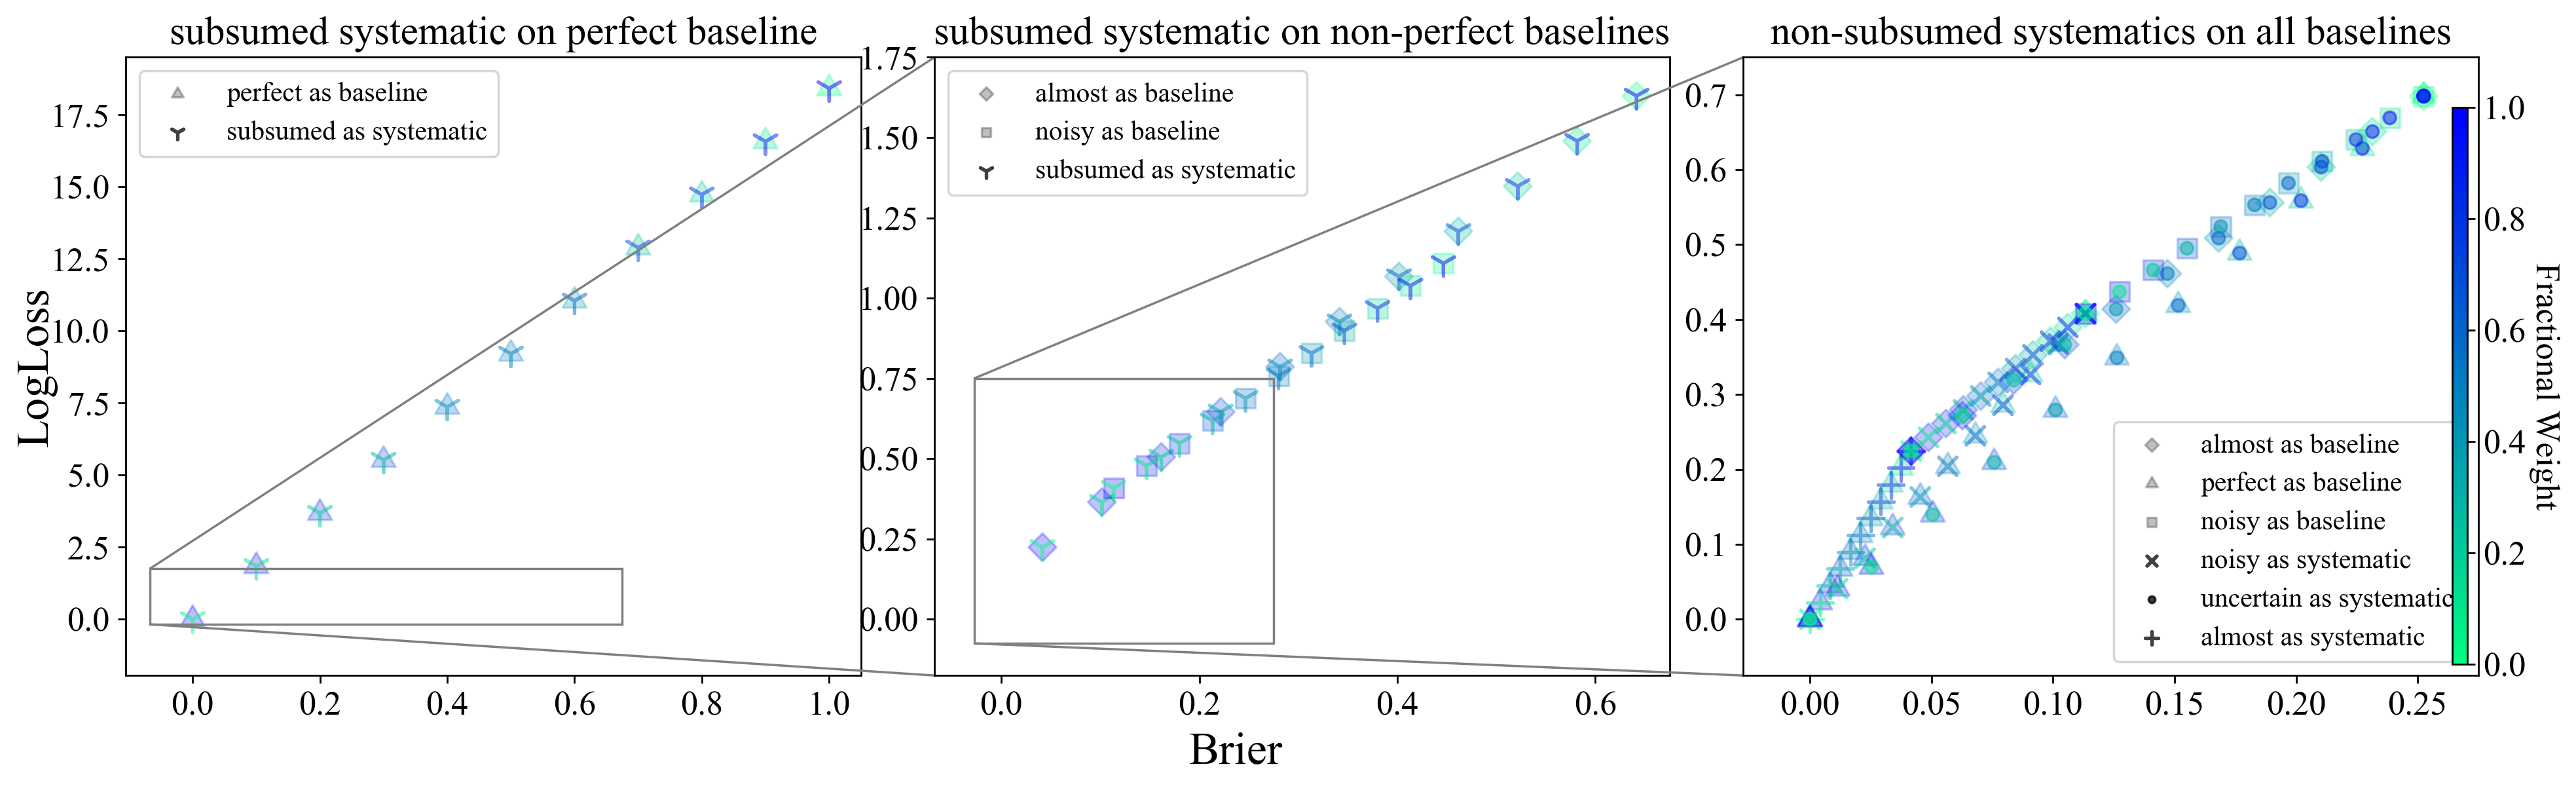
\includegraphics[width=0.99\textwidth]{./fig/multipanel_res.png}
		\caption{Weighted log-loss and Brier scores for baseline classifiers with combinations of systematics.
		Each point represents a classifier with baseline behavior (regular polygon marker) for all but one class with a particular systematic (asterisk markers).
		The color of the systematic effect and baseline behavior markers indicates the weight on the class affected by the systematic and the integrated weight evenly distributed over other classes with baseline behavior, respectively.
		Both metrics are shown in three regimes of sensitivity: to the subsumed systematic on a perfect baseline is highest, all other baselines with the subsumed systematic, and all other systematics.
		The ranges of Brier score and log-loss values between the panels are in ratios of approximately $10:7:3$ and $100:10:5$, respectively, indicating the log-loss's higher sensitivity to the presence of systematics.
		}
	\end{center}
	\label{fig:all_combined}
\end{figure*}

We demonstrate the behavior of the metrics with classification posteriors derived from conditional probability matrices composed of pairs of the characteristic classifiers of Section~\ref{sec:mockdata} is shown in Figure~\ref{fig:all_combined}.
The systematics introduced to each baseline are those that we intuitively expect to worsen performance;
the uncertain, almost perfect, noisy, and subsuming classifiers are anticipated to worsen an otherwise perfect classifier;
the uncertain, noisy, and subsuming classifiers are anticipated to worsen an otherwise almost perfect classifier;
and the uncertain and subsuming classifiers are anticipated to worsen an otherwise noisy classifier.
In every case, we apply the systematic to one true class, i.e. transforming one row of the baseline conditional probability matrix.
The metrics are evaluated at a number of weights $w$ on the affected class, with the weights on the remaining baseline classes equal to one another at $(1 - w) / (M - 1)$.
The weight values range from $0$ (all weight on the baseline) to $1$ (all weight on the systematic) at intervals of $0.1$.
This variation in weights establishes linear relationships between the log-loss and Brier score metrics for each pair of baseline and systematic.

Figure~\ref{fig:all_combined} confirms that for all weight on the perfect classifier, the values of both metrics vanish to zero.
It is immediately evident that the log-loss has more dynamic range than the Brier score overall, and that the log-loss is acutely sensitive to the subsuming systematic on a baseline of a perfect classifier.
In fact, the log-loss value for a classifier that subsumes a class into one that is classified perfectly should actually be infinite if the classes unaffected by the systematic have no weight.
The finite maximum in our tests is set by the artificial zero point established for numerical stability.
Because the combination of a subsuming classifier with a perfect baseline (left panel) is so different from all other combinations, we separate the subsuming systematic on all other baselines (middle panel) from all other systematics (right panel) in Figure~\ref{fig:all_combined}.
The dynamic range of the log-loss remains higher even outside the regime where it tends toward infinity.
The extent of the values of both metrics is higher in the middle panel with the subsuming systematic on various baselines than in the right panel with all other systematics.
This shows that both metrics are still more sensitive to the subsuming systematic than any other systematic, confirming that both can appropriately penalize the cruise control effect.

\begin{table}[]
\begin{tabular}{lll}
Classifier characteristic & Brier score & Log-loss\\
\hline
Perfect & 0.0 & 0.0\\
Almost perfect & 0.042 & 0.225\\
Noisy & 0.113 & 0.408\\
Uncertain & 0.253 & 0.699\\
Subsumed from Noisy & 0.447 & 1.109\\
Subsumed from Almost & 0.641 & 1.629\\
Subsumed from Perfect & 1.0 & 18.421\footnote{The entry for the log-loss of a classifier that subsumes a class into one that is otherwise perfectly classified should be infinite but is bounded by the numerical precision of our calculations.}
\end{tabular}
\caption{The value of each metric when the weight is entirely on the class(es) with the indicated characteristic.}
\label{tab:extents}
\end{table}

When all weight is on the class affected by a systematic, there is a characteristic limit for each metric's values, shown in Table~\ref{tab:extents}.
Because a subsumed class takes the conditional probability vector of the subsuming class, the metric values depend on what systematics may be affecting the subsuming class as well.
Based on Table~\ref{tab:extents}, both metrics would agree on the ranking of these classifiers, though this agreement is not in general guaranteed.
Furthermore, this invariant ranking is consistent with our intuition about the severity of anticipated faults of classifiers.

\begin{table}[]
\begin{tabular}{l|llll}
	& Systematics & & &\\
Baselines & Subsumed & Uncertain & Noisy & Almost\\
\hline
Perfect & 18.421 & 2.763 & 3.601 & 5.387\\
Almost perfect & 2.343 & 2.246 & 2.556 & \\
Noisy & 2.102 & 2.085 & &
\end{tabular}
\caption{The slopes for each baseline-plus-systematic pair in the space of log-loss  versus Brier score.
A higher slope corresponds to increased sensitivity of the log-loss.}
\label{tab:slopes}
\end{table}

The relative sensitivity ratios of the log-loss to the Brier score are the slopes in the trends of Figure~\ref{fig:all_combined} and are given in Table~\ref{tab:slopes}.
The log-loss always has higher sensitivity than the Brier score, particularly to the difference between the perfect classifier and any lesser classifier.
A possible implication of this behavior is that the log-loss may have an enhanced ability to distinguish between multiple high-performing classifiers that might not have meaningfully different metric values under the Brier score.
In a sense, it means that the log-loss is more susceptible to the tunnel vision classifier, with a significant response to any move toward perfection.
% Heavily unequal weighting can incentivize tunnel vision classification.
% However, the slope is higher for the almost perfect systematic than the noisy systematic, and higher for the noisy systematic than the uncertain systematic; this means that a tunnel vision classifier is deprived of the metric's favor more if it neglects other classes than if it already does fairly well for them, a case in which we would not call it much of a systematic.

% \aim{Still reworking past here.}
% Consider a weighting of $\sim0.8$ for a class affected by tunnel vision, leaving $\sim0.2$ to be shared evenly among all other classes uniformly affected by the other systematics.
% Qualitatively, we would say that a classifier that is almost perfect for other classes is superior to one that is noisy, and a classifier that is noisy for other classes is still superior to one that is uniform; furthermore, the subsuming classifier is even more harshly penalized in this situation than the uncertain classifier, meaning both metrics are  consistent with our basic tests of intuition in this case.
% However, this observation also indicates that the tunnel vision systematic is difficult to penalize, and that if the affected class is given a large weight, it can easily dominate the metric.
% If all classes are of scientific importance, heavily unequal weighting can incentivize tunnel vision classification.

% We introduced weighting of per-class metrics to discourage `tunnel vision' and `cruise control' classifiers that can ignore classes other than the most common and nonetheless perform well by a metric.
% Figure~\ref{fig:popweight} shows the impact of weighting the per-class metrics by the number of objects in the class as each is affected by one of the systematics and the other classes are held at the more realistic almost perfect performance.
% The points show different classification schemes, and all points are coloured by the change in the weighting, dependent on the size of the population class being classified.
% Conversely, the cruise control classifier and, to a lesser degree the noisy classifier, always has high log-loss and Brier score values regardless of the weight on the affected class.

% \begin{figure}
% 	\begin{center}
% 		\includegraphics[width=0.5\textwidth]{./fig/all_effects_isolated.png}
% 		\caption{Population-weighted log-loss and Brier scores for classifiers with one class affected by a systematic, as a function of the population of the affected class.
% 		Each point corresponds to an almost perfect classifier that with one class instead affected by a systematic (shape), with log-loss on the $y$ axis and Brier score on the $x$ axis.
% 		The metrics are calculated with a weighting (color and size) proportional to the log of its weight in a weighted average following Equation~\ref{eq:weightavg}.
% 		}
% 	\end{center}
% 	\label{fig:popweight}
% \end{figure}

% The tunnel vision classifier has a consistently low value under the Brier score and log-loss metric (bottom left corner of the plot), only increasing its Brier score once the weighting drops (less blue).
% In this view, the Brier score appears to be more susceptible to tunnel vision than the log-loss, demonstrating a more significant decrease as the size of the affected class increases, but both metrics have concerning behavior in this regard.
% This finding suggests that weighting alone may not be sufficient to counter the influence of this effect, and indicates a need for another balancing mechanism, such as requiring a threshold metric value on all classes.
% When considering a method of converting from one of these metrics to a finall `winner' of the classification challenge, care must be taken to ensure that all approaches do reasonably well at classifying more than one object.
% This thresholding procedure is discussed in the text

% \textbf{Ashish to reaplce/add more here?}
%\aim{Preliminary results indicate weighting will be very important for preventing the tunnel vision classifier from winning. It may be necessary to a priori anticipate which classes will have to be most strongly protected from this systematic via upweighting them.}

%\begin{figure}
%	\begin{center}
%		% \includegraphics[width=0.5\textwidth]{./fig/systematics_onlyperfect.png}
%		\caption{\aim{After much iteration on how best to present these tests, a figure similar to Figure~\ref{fig:cruise} but for the tunnel vision classifier (heading) on different baseline classifications (panels) as a function of weight on the affected class (rather than number of classes) is under construction.}}
%		\label{fig:tunnel}
%	\end{center}
%\end{figure}

\subsection{Representative classifications}
\label{sec:realresults}

\begin{table*}[]
	\begin{centering}
\begin{tabular}{lllllll}%ll}
Rank $R$ & $R_\mathrm{FoM}$ & FoM & %$R_\mathrm{AUC}$ & AUC &
$R_\mathrm{LogLoss}$ & Log-loss & $R_\mathrm{Brier}$ & Brier \\
\hline
1  & TBDT & 0.635  %& TBDT & 0.982
& TBDT & 0.0907 & TBDT & 0.0486 \\
2  & WBDT & 0.591  %& WBDT & 0.978
& TSVM & 0.113  & TSVM & 0.0583 \\
3  & TSVM & 0.514  %& TSVM & 0.969
& TNN  & 0.125  & TNN  & 0.0650 \\
4  & WSVM & 0.499  %& WSVM & 0.968
& WSVM & 0.1316 & WBDT & 0.0689 \\
5  & TNN  & 0.496  %& TNN  & 0.954
& WBDT & 0.1321 & WSVM & 0.0730 \\
6  & WNN  & 0.480  %& WNN  & 0.946
& TKNN & 0.146  & WNN  & 0.0750 \\
7  & TKNN & 0.384  %& TKNN & 0.942
& WNN  & 0.152  & TKNN & 0.0787 \\
8  & TNB  & 0.340  %& WKNN & 0.894
& WKNN & 0.228  & TNB  & 0.105  \\
9  & WKNN & 0.114  %& TNB  & 0.879
& TNB  & 0.251  & WKNN & 0.132  \\
10 & WNB  & 0.0365 %& WNB  & 0.850
& WNB  & 0.443  & WNB  & 0.178  \\
\end{tabular}
	\caption{The values of three metrics for each of ten \snmachine\ classifiers with equal weight per object.
	The metrics broadly agree on the ranking of the classifiers, confirming consistency between a conventional metric of classification performance and the metrics of probabilistic classifications presented here.
	However, there are some differences with pairwise swapping between the log-loss and Brier rankings and some significant reordering of ranks 2 through 5 with the FoM metric relative to the probabilistic metrics.}
	\label{tab:snmachineresults}
	\end{centering}
\end{table*}

We present in Table~\ref{tab:snmachineresults} the values of all metrics we considered, under equal weight per object, for classification probabilities derived from running the algorithms of \citet{lochner_photometric_2016} on the \snphotcc\ data of Section~\ref{sec:realdata}.
Table~\ref{tab:snmachineresults} also contains the ranking of classifier performance under each metric.

The FOM of Section~\ref{sec:science} differs more from the Brier and log-loss metrics than they do from one another, yet all three metrics are in agreement over the winners and losers, indicating that both of the potential \plasticc\ metrics are roughly consistent with our intuition about what makes a good classifier.
However, this agreement is not universal; the classifiers do not agree with one another on the entire ranking and could thus potentially disagree about the winner.


\section{Discussion}
\label{sec:discussion}

The goal of this work is to identify the metric most suited to \plasticc, which seeks classification posteriors of complete light curves similar to those anticipated from \lsst, with an emphasis on classification over all types, rewarding a ``best in show'' classifier rather than focusing on any one class or scientific application.\footnote{At the conclusion of \plasticc, other metrics specific to scientific uses of one or more particular classes will be used to identify ``best in class'' classification procedures that will be useful for more targeted science cases.}
The weighted log-loss is thus the metric most suited to the current \plasticc\ release.

% \sout{Future releases of \plasticc\ will focus on different challenges in transient and variable object classification, with metrics appropriate to identifying methodologies that best enable those goals.
% We discuss approaches to identifying optimal metrics for these variations, which may be developed further in future work.}
\changes{Because transient and variable object classification is crucial for a variety of scientific objectives, the impact of a shared performance metric on this diversity of goals leads to complex and covariant trade-offs.
Though the selection criteria for metrics specific to each science goal are outside the scope of this work, which concerns only the first instantiation of \plasticc, we discuss below some issues concerning the identification of metrics for a few example science cases.}

\subsection{\changes{Ongoing transient follow-up}}
\label{sec:early}

Spectroscopic follow-up is only expected of a small fraction of \lsst's detected transients and variable objects due to limited resources for such observations.
In addition to optical spectroscopic follow-up, photometric observations in other wavelength bands (near infrared and x-ray from space; microwave and radio from the ground) \changes{or at different times} will be key to building a physical understanding of the object, particularly as we enter the era of multi-messenger astronomy with the added possibility of optical gravitational wave signatures.
Prompt follow-up observations are highly informative for fitting models to the light curves of familiar source classes and to characterizing anomalous light curves that could indicate never-before-seen classes that have eluded identification due to rarity or faintness.
As such, decisions about follow-up resource allocation must be made quickly and under the constraint that resources wasted on a misclassification consume the budget remaining for future follow-up attempts.
A future version of \plasticc\ focused on early light curve classification should have a metric that accounts for these limitations and rewards classifiers that perform better even when fewer observations of the lightcurve are available.

We consider the decision of whether to initiate follow-up observations to be binary and deterministic.
However, it is possible to conceive of non-binary decisions about follow-up resources; for example, one could choose between dedicating several hours on a spectroscopic instrument following up on one likely candidate or dedicating an hour each on several less likely candidates.
Here, we will discuss a metric for an early classification challenge to be focused on deterministic classification because the conversion between classification posteriors and decisions is uncharted territory that we do not explore at this time.

Even within the scope of spectroscopic follow-up as a primary motivation for early light curve classification, the goals of model-fitting to known classes and discovery of new classes would likely not share an optimal metric.
The critical question for choosing the most appropriate metric for any specific science goal motivating follow-up observations is to maximize information.
We provide two examples of the kind of information one must maximize via early light curve classification and the qualities of a deterministic metric that might enable it.

\subsection{\changes{Spectroscopic supernova cosmology}}
\label{sec:spec_sncosmo}

Supernova cosmology with spectroscopically confirmed light curves benefits from true positives, which contribute to the constraining power of the analysis by including one more data point;
when the class in which one is interested is as plentiful as SN Ia and our resources limited a priori, we may not be concerned by a high rate of false negatives.
% requires making a decision balancing the improved constraining power of including another SN Ia in the analysis, thereby constraining the cosmological parameters, so only true positives contribute information, and if we had a perfect classifier and standard follow-up spectroscopy resources, there would be a maximum amount of information about the cosmological parameters that could be gained in this way.
% Each false positive uses the same resources but adds no information about the cosmological parameters, and each false negative consumes no follow-up resources and deprives the Hubble diagram of one more data point.
False positives, on the other hand, may not enter the cosmology analysis, but they consume follow-up resources, thereby depriving the endeavor of the constraining power due to a single SN Ia.

A perfect classifier would lead to a maximum amount of information about the cosmological parameters conditioned on the follow-up resource budget.
% \sout{For this scientific application, the metric must be chosen to balance the value of the information forgone by a false positive and the value of information forgone by a false negative, and the value placed on these is effectively weighted by the value we as researchers place on follow-up resources.}
\changes{Consider deterministic labels derived from cutoffs in probabilistic classifications for this scientific application; raising the probability cutoff reduces the number of false positives, boosting the cosmological constraining power, but at a cost of increasing the number of false negatives, which represent constraining power forgone.
As this tradeoff is asymmetric, it is insufficient to consider only the true and false positive and negative rates, as the \snphotcc\ FoM does, without propagating their impact on the information gained about the cosmological parameters.}
% \aim{Cite some deterministic metrics relating to TP/FP?}

\subsection{\changes{Anomalous transient and variable detection}}
\label{sec:anom}

\changes{A particularly exciting science case is anomaly detection, the discovery of entirely unknown classes of transient or variable astrophysical sources, or distinguishing some of the rarest types of sources from more abundant types.
Like the case of spectroscopic supernova cosmology discussed above,} anomaly detection also gains information only from true positives, but the cost function is different in that the potential information gain is unbounded when there is no prior information about undiscovered classes.
% \aim{COMMENT RB: not to stay in doc, but I don't understand the prev sentence. I would also object to the recent detection of kilonova as a good example of anomaly detection, I can buy it if I squint very hard
% COMMENT AIM: Agreed, but I couldn't think of a better one at the time of writing.}
% \sout{An example would be the recent detection of a kilonova, flagged initially by the detection of gravitational waves from an object.}
\changes{The discovery of pulsars serves as an example of novelty detection enabled by a human classifier \citep{hewish_observation_1968, bell_burnell_measurement_1969}.}

Resource availability for identifying new classes is more flexible, increasing when new predictions or promising preliminary observations attract attention, and decreasing when a discovery is confirmed and the new class is established.
In this way, a false positive does not necessarily consume a resource that could otherwise be dedicated to a true positive, and the potential information gain is sufficiently great that additional resources would likely be allocated to observe the potential object.
% A false negative, on the other hand, represents forgoing an unbounded quantity of information, so minimizing the false negative rate is as important as maximizing the true positive rate.
% For a rare event like a kilonova, a false negative represents an unbounfalse positive does not appreciably reduce the amount of remaining information available to collect, but a false negative represents a large quantity of information forgone.
% Furthermore, r
% In this case, the information forgone by a false negative is significant compared to the information forgone by a false positive.
Thus, a metric \changes{for evaluating} anomaly detection \changes{effectiveness} would aim to \changes{minimize the false negative rate and maximize the true positive rate.}
% \aim{Cite some deterministic metrics relating to TP/FN?}

% \subsection{Hierarchical classes}
% \label{sec:hierarchical}
%
% \aim{TODO: We would like to at some point add some content on possible ideas for extending metrics to hierarchical classes, namely conditional extensions of log-loss and possible drawbacks of penalization that can be compensated for by weighting, as well as the challenge that could pose for interpretation.}

\subsection{Difficult light curve classification}
\label{sec:difficult}

Photometric light curve classification may be challenging for a number of reasons, including the sparsity and irregularity of observations, the possible classes and how often they occur, and the distances and brightnesses of the sources of the light curves.
These factors may represent limitations on the information content of the light curves, but appropriate classifiers may be able to overcome them to a certain degree.

Though quality cuts can eliminate the most difficult light curves from entering samples used for science applications, such a practice discards information that may be of value under an analysis methodology leveraging the larger number of light curves included in a sample without cuts.
Thus, classification methods that perform well on light curves characterized by lower signal-to-noise ratios are specially important for exploiting the full potential of upcoming surveys like \lsst.

This version of \plasticc\ implements quality cuts to homogenize difficulty to some degree, and notions of classification difficulty may depend on information that will not be available until after the challenge concludes.
While the groundwork for a metric incorporating data quality has been laid by \citet{wu_radio_2018}, we defer to future work an investigation of this possibility.


\section{Conclusion}
\label{sec:conclusion}

% intro and data
As part of the preparation for \plasticc\, we investigated the properties of metrics suitable for probabilistic light curve classifications in the absence of a single scientific goal.
Therefore, we sought a metric that avoids reducing classification probabilities to deterministic labels \changes{and is compatible with a multi-class, rather than binary (two-class), setting.
We did not consider some of the most popular metrics used in astronomy (such as accuracy, combinations of the true and false positive and negative rates, and AUC functions thereof) because they did not satisfy these criteria, even though it is in principle possible to extend such metrics for our situation.}
% In line with the goals of \plasticc, an important desideratum was to have a metric that tends to} reward a classifier's performance across all classes over a classifier that performs well on a small subset of the classes and poorly on others.
\changes{Our experimental design thus explores the response of potential metrics to simulated classification submissions from a set of mock classifier archetypes expected of generic transient and variable classifiers.}

% the metrics
\changes{We identified two metrics of multi-class classification probabilities established in the literature: the Brier score and the log-loss.}
The Brier score and the log-loss metrics are structurally and conceptually different, with wholly different interpretations.
The Brier score is a sum of square differences between probabilities;
the explicit penalty term is an attractive feature, but it treats probabilities as generic scores.
The log-loss on the other hand is readily interpretable \changes{as a measure of information}, meaning the metric itself could be propagated into forecasting the cosmological constraining power of \lsst, affecting the choice of observing strategy.

% weights
\changes{When evaluated with equal weight on each classified object,} both the Brier score and the log-loss metrics are susceptible to rewarding a classifier that performs well on the most prevalent class and poorly on all others, which fails to meet the needs of \plasticc's diverse motivations \changes{under the unavoidable population imbalances of astronomical data}.
\changes{To discourage competitors from neglecting rare classes,} we explored a weighted average of the metric values on a per-class basis as a possible mitigation strategy to incentivize classifying uncommon classes, effectively ``leveling the playing field'' in the presence of highly nonuniform class membership.
%\changes{%Such weights were taken to be the same for all objects in the same class.

% findings
On the basis of the mock classifier rankings, we found that both metrics reward the classifiers that are better and penalize those that are worse, where better and worse are defined by our common intuition, yielding the same rankings under either metric and demonstrating that both could be appropriate for \plasticc.
However, since only one could be selected, the log-loss was chosen due to its potential for interpretation after the conclusion of the challenge.
\changes{While modifyinging the log-loss metric to handle weights for different classes diminishes its interpretability, it can still be understood as information gain, subject to the value we as scientists place on knowledge of each class.}

% justifying limited choice of metrics to consider
\changes{The space of possible metrics we could have considered is truly unbounded, from traditional metrics of deterministic labels to established extensions thereof for probabilistic classifications to novel quantities tuned to any given science case.
Though there was no need to do a more extensive survey of metrics nor to devise new metrics for \plasticc, since both log-loss and Brier score passed the basic sanity tests for this application, further work remains to be done in optimally selecting probabilistic classification metrics in other astronomical contexts.}

We conclude by noting that care should be taken in planning future open challenges to ensure alignment between the challenge goals and the performance metric, so that efforts are best directed to achieve the challenge objectives.
It is our hope hope that this study of metric performance across a range of systematic effects and weights may serve as a guide to approaching the problem of identifying promising probabilistic classifiers for general science applications.


% ----------------------------------------------------------------------

\subsection*{Acknowledgments}

%%% Here is where you should add your specific acknowledgments, remembering that some standard thanks will be added via the \code{desc-tex/ack/*.tex} and \code{contributions.tex} files.


 % Standard papers only: author contribution statements. For examples, see http://blogs.nature.com/nautilus/2007/11/post_12.html

% This work used TBD kindly provided by Not-A-DESC Member and benefitted from comments by Another Non-DESC person.

% Standard papers only: A.B.C. acknowledges support from grant 1234 from ...
This paper has undergone internal review in the LSST Dark Energy Science Collaboration. % REQUIRED if true
The authors would like to thank Melissa Graham, Weikang Lin, and Chad Schafer for serving as the LSST-DESC publication review committee.
The authors further wish to thank Kaisey Mandel, Tom Loredo, Rick Kessler, and Lluis Galbany for helpful feedback provided in the preparation of this paper.

AIM is advised by David W. Hogg and was supported by National Science Foundation grant AST-1517237.
TA is supported in part by STFC.

RB and CS are supported by the Swedish Research Council (VR) through the Oskar Klein Centre.
Their work was further supported by the research environment grant ``Gravitational Radiation and Electromagnetic Astrophysical Transients (GREAT)'' funded by the Swedish Research council (VR) under Dnr 2016-06012.

The financial assistance of the National Research Foundation (NRF) towards this research is hereby acknowledged.
Opinions expressed and conclusions arrived at, are those of the authors and are not necessarily to be attributed to the NRF.
This work is partially supported by the European Research Council under the European Community’s Seventh Framework Programme (FP7/2007-2013)/ERC grant agreement no 306478-CosmicDawn.

Canadian co-authors acknowledge support from the Natural Sciences and Engineering Research Council of Canada.
The Dunlap Institute is funded through an endowment established by the David Dunlap family and the University of Toronto.
The authors at the University of Toronto acknowledge that the land on which the University of Toronto is built is the traditional territory of the Haudenosaunee, and most recently, the territory of the Mississaugas of the New Credit First Nation.
They are grateful to have the opportunity to work in the community, on this territory.

We acknowledge the University of Chicago Research Computing Center for support of this work.
This research used resources of the National Energy Research Scientific Computing Center (NERSC), a U.S. Department of Energy Office of Science User Facility operated under Contract No. DE-AC02-05CH11231.

\input{desc-tex/ack/standard} % also available: key standard_short

% The DESC acknowledges ongoing support from the Institut National de Physique Nucleaire et de Physique des Particules in France; the Science \& Technology Facilities Council in the United Kingdom; and the Department of Energy, the National Science Foundation, and the LSST Corporation in the United States.
%
% DESC uses resources of the IN2P3 Computing Center (CC-IN2P3--Lyon/Villeurbanne - France) funded by the Centre National de la Recherche Scientifique; the National Energy Research Scientific Computing Center, a DOE Office of Science User Facility supported by the Office of Science of the U.S. Department of Energy under Contract No. DE-AC02-05CH11231; STFC DiRAC HPC Facilities, funded by UK BIS National E-infrastructure capital grants; and the UK particle physics grid, supported by the GridPP Collaboration.
%
% This work was performed in part under DOE Contract DE-AC02-76SF00515.

% We acknowledge the use of An-External-Tool-like-NED-or-ADS.

%{\it Facilities:} \facility{LSST}

% Include both collaboration papers and external citations:
\bibliography{main,lsstdesc}

\end{document}

% ======================================================================
